% Customizable fields and text areas start with % >> below.
% Lines starting with the comment character (%) are normally removed before release outside the collaboration, but not those comments ending lines

% svn info. These are modified by svn at checkout time.
% The last version of these macros found before the maketitle will be the one on the front page,
% so only the main file is tracked.
% Do not edit by hand!
\RCS$Revision: 134703 $
\RCS$HeadURL: svn+ssh://svn.cern.ch/reps/tdr2/notes/SMP-12-013/trunk/SMP-12-013.tex $
\RCS$Id: SMP-12-013.tex 134703 2012-07-04 06:35:38Z dmytro $
%%%%%%%%%%%%% local definitions %%%%%%%%%%%%%%%%%%%%%
% This allows for switching between one column and two column (cms@external) layouts
% The widths should  be modified for your particular figures. You'll need additional copies if you have more than one standard figure size.
\newlength\cmsFigWidth
\ifthenelse{\boolean{cms@external}}{\setlength\cmsFigWidth{0.85\columnwidth}}{\setlength\cmsFigWidth{0.4\textwidth}}
\ifthenelse{\boolean{cms@external}}{\providecommand{\cmsLeft}{top}}{\providecommand{\cmsLeft}{left}}
\ifthenelse{\boolean{cms@external}}{\providecommand{\cmsRight}{bottom}}{\providecommand{\cmsRight}{right}}
%%%%%%%%%%%%%%%  Title page %%%%%%%%%%%%%%%%%%%%%%%%
\cmsNoteHeader{SMP-12-013} % This is over-written in the CMS environment: useful as preprint no. for export versions
% >> Title: please make sure that the non-TeX equivalent is in PDFTitle below
\title{Measurement of the WW production cross section 
~\\in pp collisions at $\sqrt s$ = 8~TeV}

% >> Authors
%Author is always "The CMS Collaboration" for PAS and papers, so author, etc, below will be ignored in those cases
%For multiple affiliations, create an address entry for the combination
%%% \address[neu]{Northeastern University}
%%% \address[fnal]{Fermilab}
%%% \address[cern]{CERN}
\author[cern]{The CMS Collaboration}

% >> Date
% The date is in yyyy/mm/dd format. Today has been
% redefined to match, but if the date needs to be fixed, please write it in this fashion.
% For papers and PAS, \today is taken as the date the head file (this one) was last modified according to svn: see the RCS Id string above.
% For the final version it is best to "touch" the head file to make sure it has the latest date.
\date{\today}

% >> Abstract
% Abstract processing:
% 1. **DO NOT use \include or \input** to include the abstract: our abstract extractor will not search through other files than this one.
% 2. **DO NOT use %**                  to comment out sections of the abstract: the extractor will still grab those lines (and they won't be comments any longer!).
% 3. **DO NOT use tex macros**         in the abstract: External TeX parsers used on the abstract don't understand them.
\abstract{
This document reports on a measurement of the W$^+$W$^-$ production
cross section in pp collisions at $\sqrt{s} = $ 8~TeV. The data were
collected at the LHC with the CMS detector, and correspond to an
integrated luminosity of 3.54~fb$^{-1}$. The W$^+$W$^-$ candidates are
selected in events with two charged leptons (electrons or muons) and
large missing transverse energy. The W$^+$W$^-$ cross section is
measured to be $69.9 \pm 2.8$~(stat.)~$\pm5.6$~(syst.)~$\pm 3.1$~(lumi.)~pb.

}

% >> PDF Metadata
% Do not comment out the following hypersetup lines (metadata). They will disappear in NODRAFT mode and are needed by CDS.
% Also: make sure that the values of the metadata items are sensible and are in plain text (no TeX! -- for \sqrt{s} use sqrt(s) -- this will show with extra quote marks in the draft version but is okay).

\hypersetup{%
pdfauthor={WW Group},%
pdftitle={Measurement of WW production rate},%
pdfsubject={CMS},%
pdfkeywords={CMS, physics, software, computing}}

\maketitle %maketitle comes after all the front information has been supplied

% >> Text
%%%%%%%%%%%%%%%%%%%%%%%%%%%%%%%%  Begin text %%%%%%%%%%%%%%%%%%%%%%%%%%%%%
%% **DO NOT REMOVE THE BIBLIOGRAPHY** which is located before the appendix.
%% You can take the text between here and the bibiliography as an example which you should replace with the actual text of your document.
%% If you include other TeX files, be sure to use "\input{filename}" rather than "\input filename".
%% The latter works for you, but our parser looks for the braces and will break when uploading the document.
%%%%%%%%%%%%%%%
\newcommand{\CLs}{\ensuremath{CL_\mathrm{s}}}
\newcommand{\CLb}{\ensuremath{CL_\mathrm{b}}}
\newcommand{\CLsb}{\ensuremath{CL_\mathrm{s+b}}}

%\newcommand{\GeV}{\ensuremath{\mathrm{Ge\kern -0.1em V}}}
%\newcommand{\TeV}{\ensuremath{\mathrm{Te\kern -0.1em V}}}
%\newcommand{\TeVcc}{\ensuremath{\,\mathrm{Te\kern -0.1em V\!/c}^2}}
%\newcommand{\GeVcc}{\ensuremath{\,\mathrm{Ge\kern -0.1em V\!/c}^2}}
%\newcommand{\MeVcc}{\ensuremath{\,\mathrm{Me\kern -0.1em V\!/c}^2}}
%\newcommand{\GeVc}{\ensuremath{\mathrm{Ge\kern -0.1em V}\!/c}}
\newcommand{\nanob}{\mbox{{\rm ~nb}~}}
\newcommand{\fb}{\ensuremath{\mathrm{fb}}}
\newcommand{\pb}{\ensuremath{\mathrm{pb}}}
\newcommand{\ifb}{\ensuremath{\mathrm{fb^{-1}}}}
\newcommand{\ipb}{\ensuremath{\mathrm{pb^{-1}}}}
\newcommand{\grad}{\ensuremath{^{\circ}}}
%
% Special user made math symbols
%
\newcommand{\lsim}{\raisebox{-1.5mm}{$\:\stackrel{\textstyle{<}}{\textstyle{\sim}}\:$}}
\newcommand{\gsim}{\raisebox{-1.5mm}{$\:\stackrel{\textstyle{>}}{\textstyle{\sim}}\:$}}

% particles

\newcommand{\pipm}{\ensuremath{\pi^{\pm}}}
\newcommand{\pizero}{\ensuremath{\pi^{0}}}
\newcommand{\Hi}{\ensuremath{\mathrm{H}}}
\newcommand{\W}{\ensuremath{\mathrm{W}}}
\newcommand{\Wjets}{\ensuremath{\mathrm{W+jets}}}
\newcommand{\Zjets}{\ensuremath{\mathrm{Z+jets}}}
\newcommand{\Wt}{\ensuremath{\mathrm{Wt}}}
\newcommand{\Wstar}{\ensuremath{\mathrm{W}^{*}}}
\newcommand{\Wparenthesisstar}{\ensuremath{\mathrm{W}^{(*)}}}
\newcommand{\WW}{\ensuremath{\W^+\W^-}}
%\newcommand{\Z}{\ensuremath{\mathrm{Z}}}
\newcommand{\Zstar}{\ensuremath{\mathrm{Z}^{*}}}
\newcommand{\ZZ}{\ensuremath{\Z\Z}}
\newcommand{\WZ}{\ensuremath{\W\Z}}
\newcommand{\El}{\ensuremath{\mathrm{\mathrm{e}}}}
\newcommand{\Elp}{\ensuremath{\mathrm{\mathrm{e}}^{+}}}
\newcommand{\Elm}{\ensuremath{\mathrm{\mathrm{e}}^{-}}}
\newcommand{\Elpm}{\ensuremath{\mathrm{\mathrm{e}}^{\pm}}}
\newcommand{\Elmp}{\ensuremath{\mathrm{\mathrm{e}}^{\mp}}}
\newcommand{\M}{\ensuremath{\mu}}
\newcommand{\Mp}{\ensuremath{\mu^{+}}}
\newcommand{\Mm}{\ensuremath{\mu^{-}}}
\newcommand{\Mpm}{\ensuremath{\mu^{\pm}}}
\newcommand{\Mmp}{\ensuremath{\mu^{\mp}}}
\newcommand{\Tau}{\ensuremath{\tau}}
\newcommand{\Nu}{\ensuremath{\nu}}
\newcommand{\Nubar}{\ensuremath{\bar{\nu}}}
\newcommand{\Lep}{\ensuremath{\mathrm{\ell}}}
\newcommand{\Lepp}{\ensuremath{\mathrm{\ell}^{+}}}
\newcommand{\Lepm}{\ensuremath{\mathrm{\ell}^{-}}}
\newcommand{\Lprime}{\ensuremath{\Lep^{\prime}}}
\newcommand{\Prot}{\ensuremath{\mathrm{p}}}
\newcommand{\Pbar}{\ensuremath{\bar{\mathrm{p}}}}
\newcommand{\PP}{\Prot\Prot}
\newcommand{\PPbar}{\Prot\Pbar}
%\newcommand{\ttbar}{\ensuremath{\mathrm{t}\bar{\mathrm{t}}}}
\newcommand{\qq}{\ensuremath{\mathrm{q}\mathrm{q}}}
%\newcommand{\bbbar}{\ensuremath{\mathrm{b}\bar{\mathrm{b}}}}
\newcommand{\Wtb}{\ensuremath{\W\mathrm{t}\mathrm{b}}}
\newcommand{\Top}{\ensuremath{\mathrm{t}}}
\newcommand{\Bot}{\ensuremath{\mathrm{b}}}
\newcommand{\Atop}{\ensuremath{\bar{\mathrm{t}}}}
\newcommand{\Abot}{\ensuremath{\bar{\mathrm{b}}}}
% arrow
\newcommand{\To}{\ensuremath{\rightarrow}}

% masses
\newcommand{\mHi}{\ensuremath{m_{\mathrm{H}}}}
\newcommand{\mW}{\ensuremath{m_{\mathrm{W}}}}
\newcommand{\mZ}{\ensuremath{m_{\mathrm{Z}}}}
\newcommand{\mll}{\ensuremath{m_{\Lep\Lep}}}

% kinematics
% \newcommand{\pt}{\ensuremath{p_\mathrm{T}}}
\newcommand{\ptveto}{\ensuremath{\pt^\mathrm{veto}}}
\newcommand{\ptl}{\ensuremath{p_\perp^{\Lep}}}
\newcommand{\ptlmax}{\ensuremath{p_{\mathrm{T}}^{\Lep,\mathrm{max}}}}
\newcommand{\ptlmin}{\ensuremath{p_{\mathrm{T}}^{\Lep,\mathrm{min}}}}
\newcommand{\met}{\ensuremath{\Et^{\mathrm{miss}}}}
\newcommand{\delphill}{\ensuremath{\Delta\phi_{\Lep\Lep}}}
\newcommand{\deletall}{\ensuremath{\Delta\eta_{\Lep\Lep}}}
\newcommand{\delphimetl}{\ensuremath{\Delta\phi_{\met\Lep}}}
\newcommand{\Et}{\ensuremath{E_\mathrm{T}}}
\newcommand{\delR}{\ensuremath{\Delta R}}
\newcommand{\Eta}{\ensuremath{\eta}}
\newcommand{\GAMMA}{\ensuremath{\gamma}}

%efficiencies
\newcommand{\effsig}{\ensuremath{\varepsilon_{\mathrm{bkg}}^{\mathrm{S}}}}
\newcommand{\effnorm}{\ensuremath{\varepsilon_{\mathrm{bkg}}^{\mathrm{N}}}}
\newcommand{\Nsig}{\ensuremath{N_{\mathrm{bkg}}^{\mathrm{S}}}}
\newcommand{\Nnorm}{\ensuremath{N_{\mathrm{bkg}}^{\mathrm{N}}}}

% processes
\newcommand{\dyee}{\ensuremath{\mathrm{\Z}/\GAMMA^*\mathrm{\to e^+e^-}}}
\newcommand{\dymm}{\ensuremath{\mathrm{\Z/}\GAMMA^*\to\mu^+\mu^-}}
\newcommand{\dytt}{\ensuremath{\mathrm{\Z}/\GAMMA^* \to\tau^+\tau^-}}
\newcommand{\dyll}{\ensuremath{\mathrm{\Z}/\GAMMA^*\mathrm{\to \ell^+\ell^-}}}
\newcommand{\zee}{\ensuremath{\mathrm{\Z\to e^+e^-}}}
\newcommand{\zmm}{\ensuremath{\mathrm{\Z}\to\mu^+\mu^-}}
\newcommand{\ztt}{\ensuremath{\mathrm{\Z}\to\tau^+\tau^-}}
\newcommand{\zll}{\ensuremath{\mathrm{\Z\to \ell^+\ell^-}}}
%\newcommand{\ttbar}{\ensuremath{t\bar{t}}}
\newcommand{\ppww}{\ensuremath{pp \to W^+W^-}}
\newcommand{\wwlnln}{\ensuremath{W^+W^-\to \ell^+\nu \ell^-\bar{\nu}}}
\newcommand{\ww}{\ensuremath{WW}}
\newcommand{\wwpm}{\ensuremath{W^+W^-}}
\newcommand{\hww}{\Hi\to\WW}
\newcommand{\wz}{\ensuremath{\W\Z}}
\newcommand{\zz}{\ensuremath{\Z\Z}}
\newcommand{\wgamma}{\ensuremath{\W\GAMMA}}
\newcommand{\wjets}{\ensuremath{\W+}jets}
\newcommand{\tw}{\ensuremath{\mathrm{t}\W}}
\newcommand{\singletopt}{\ensuremath{t} ($t$-chan)}
\newcommand{\singletops}{\ensuremath{t} ($s$-chan)}

%other
\def\fixme{({\bf FixMe})}
\newcommand{\ee}{\ensuremath{ee}}
\newcommand{\emu}{\ensuremath{e\mu}}
\def\mm{\ensuremath{\mu\mu}}

% Integrated luminosity
\newcommand{\usedLumi}{3.54~\ifb}
\newcommand{\usedLumiWithSyst}{3.54~\pm~0.16~\ifb}
% The answer
\newcommand{\measuredCrossSection}{\ensuremath{69.9 \pm 2.8~(\rm{stat.}) \pm 5.6~(\rm{syst.}) \pm 3.1~({lumi.})~\rm{pb}}}
%\newcommand{\nloCrossSection}{\ensuremath{57.25~\pb \left(^{+4.1\%}_{-2.8\%}\right)}} %%% errors in %
\newcommand{\nloCrossSection}{\ensuremath{57.3 \left(^{+2.4}_{-1.6}\right)~\pb}} %%% errors in pb
 

\section{Introduction}
\label{sec:introduction}
Studies of $\WW$ production test the description of electroweak and
strong interactions in the standard model (SM).
Next-to-leading order (NLO) calculations~\cite{MCFM} of $\WW$ production in pp
collisions at $\sqrt{s} = 8~\TeV$ predict a cross section of
%
\begin{equation}
\sigma^{{\rm NLO}} (\mathrm{gg}\to\WW + \mathrm{qq}\to\WW) = \nloCrossSection.\nonumber
\end{equation}

The dominant $\WW$ production mechanisms are the s-channel and
t-channel $\rm{q}\bar{\rm{q}}$ annihilation diagrams. The gluon-gluon fusion
contributes $\sim$3\%. The $\W\W\gamma$ and $\W\W\Z$ triple-gauge boson couplings (TGCs) in
the s-channel are sensitive to possible new physics processes at a higher mass
scale. The presence of anomalous TGCs would change the $\WW$ production rate or
kinematic distributions from the SM predictions. In addition, $\WW$ production
is an important background source for new particle searches, e.g. Higgs
boson searches~\cite{HiggsPAS2012}. In fact, the selection applied in this paper
closely follows the selection applied in the Higgs boson search in the event
category with zero counted jets.
The Higgs boson preselection for masses above 140~\GeV and the selection
applied in this paper differ only in the trailing lepton minimum transverse momentum.
This requirement is tightened from 10~\GeV to 20~\GeV
to further suppress the background from $\Wjets$ events, where the trailing 
lepton is a misidentified jet. With this selection a
SM Higgs boson with a mass of 110 (130)~\GeV would enhance the $\WW$ signal by
about $0.3\%$ $(7\%)$.

This paper reports a measurement of the $\WW$ production cross section in pp
collisions at $\sqrt{s} = 8~\TeV$, performed on a dataset corresponding to an
integrated luminosity of $\usedLumi$, collected during 2012.


\section{CMS Detector and Simulations}
\label{sec:cms}
While the CMS detector is described in detail elsewhere~\cite{CMSdetector}, the
key components for this analysis are summarized here.
A superconducting solenoid occupies the
central region of the CMS detector, providing an axial magnetic
field of 3.8~Tesla parallel to the beam direction.
The silicon pixel and strip
tracker, the crystal electromagnetic calorimeter and the brass/scintillator hadron
calorimeter are located within the solenoid. A quartz-fiber
Cherenkov calorimeter extends the coverage to $|\eta| <$ 5.0, where pseudorapidity
is defined as $\eta=-{\rm ln}[\tan{(\theta/2)}]$,
and $\theta$ is the polar angle of the trajectory of the particle
with respect to the beam direction. Muons are measured
in gas detectors embedded in the iron return yoke outside the
solenoid.
The first level of the CMS trigger system, composed of custom
hardware processors, is designed to select the most interesting events
in less than 3 $\mu$s using information from the calorimeters and muon
detectors. The High Level Trigger processor farm further
decreases the event rate to a few hundred Hz, before data storage.

This measurement is based on $\WW$ candidate events in which
both bosons decay leptonically. The experimental signature consists of
two isolated, high transverse momentum ($\pt$), 
oppositely-charged leptons (electrons or muons) and large
missing transverse energy ($\met$, defined as the modulus of the negative vector sum of the 
transverse momenta of all reconstructed particles, charged or neutral, in the event) due to the undetected neutrinos.
Several SM processes lead to backgrounds to the $\WW$ sample.
These include $\Wjets$, $\wgamma$, and ${\rm QCD}$ multi-jet events where at
least one of the jets is misidentified as a lepton, top production
($\ttbar$ and $\tw$), Drell-Yan $\dyll$, and diboson
production ($\WZ$, and $\ZZ$).

A number of Monte Carlo event generators are used to simulate the signal and
backgrounds. The $\rm{q}\bar{\rm{q}}\to\WW$ signal, $\Wjets$, $\WZ$,
$\W\gamma^{(*)}$, Drell-Yan and $\ttbar$ processes are generated using the
\textsc{madgraph}~\cite{madgraph} event generator. The $\mathrm{gg} \to \WW$
signal component, which is expected to contribute 3\% of the total $\WW$
production rate~\cite{MCFM}, is generated using \textsc{gg2ww}~\cite{ggww}.
The \textsc{powheg} program~\cite{powheg} provided event samples for the $\tw$
process, and the remaining processes are generated using \textsc{pythia}~\cite{pythia}.
For leading-order generators, the default set of parton distribution functions
(PDF) used to produce these samples is \textsc{cteq6l}~\cite{cteq66}, while 
\textsc{ct10}~\cite{ct10} is used for next-to-leading order generators.
NLO calculations are used for background cross sections.
For all processes, the detector response is simulated using a detailed
description of the CMS detector, based on the \textsc{geant4}
package~\cite{Agostinelli:2002hh}.

The simulated samples are reweighted according to the distribution of number of pp interactions 
per bunch crossing (pile-up) as measured in the data.


\section{Event Preselection}
\label{sec:ww_evtsel}
Three final states are considered:
$\Elp\Elm$, $\Mp\Mm$ and $\Elpm\Mmp$.
W$\to \ell \nu$ ($\ell = \mathrm{e},\mu$) decays are the main signal
components, while $\W\to\tau\nu_{\tau}$ events with leptonic $\tau$
decays are included, although the analysis is not optimised for this final state.
The events are selected by trigger conditions requiring
the presence of one or two high $\pt$ electrons or muons.

Two oppositely-charged lepton candidates are required, both with $\pt > 20~\GeV$.
Muon candidates~\cite{muonpas} are identified using a selection close to
the one described in Ref.~\cite{Chatrchyan:2011tz}, while
electron candidates are selected using a multivariate
approach, that exploits correlations among the selection variables
described in~\cite{egmpas} to improve identification performance. 
The lepton candidates are required to be compatible with the primary vertex of the
event, which is chosen as the vertex with highest $\sum \pt^2$ of its associated tracks. 
This criterion provides the correct assignment for the
primary vertex in more than 99\% of both signal and
background events for the pile-up distribution observed in the data. 

Charged leptons from $\W$ boson decays are usually isolated
from other activity in the event. For each lepton candidate, a cone
is constructed around the track direction at the event vertex.  The scalar
sum of the transverse energy of each reconstructed
particle~\cite{PFT-09-001} compatible with the
chosen primary vertex and contained within the cone is calculated
excluding the contribution from the lepton candidate itself. Electron candidates
are rejected if this sum exceeds 15\% of the candidate $\pt$.
Cones of several widths are constructed around the track direction at the event vertex 
to account for the differences in the differential energy deposit between a muon and a jet 
faking a lepton. This information is combined using a multivariate approach.
For both electrons and muons a correction is applied to account for the contribution to 
the energy in the isolation cone due to the several pp interactions per bunch crossing.
A median energy density ($\rho$) is determined event by event and the pile-up contribution to 
the transverse energy is estimated as the product of $\rho$ and an effective isolation cone area. 
This contribution is  subtracted~\cite{Cacciari:subtraction} from the transverse energy in the 
isolation cone.

Jets are reconstructed from calorimeter and tracker information using
the particle-flow technique~\cite{PFT-09-001,jetpas}. The anti-$\mathrm{k_T}$
clustering algorithm~\cite{antikt} with distance parameter $\mathrm{
R}=0.5$ is used, as implemented in the \textsc{fastjet}
package~\cite{Cacciari:fastjet1,Cacciari:fastjet2}. The jet energy is corrected
for pile-up in a manner similar to the correction of the energy inside a lepton
isolation cone. Jet energy corrections are also applied as a function of the jet
$\Et$ and $\eta$~\cite{cmsJEC}. 

The properties of the hard jets are modified by particles from pile-up interactions;
a combinatoric background from low-\pt jets from pile-up interactions that get 
clustered into high-\pt jets may also arise.
A multivariate selection is applied to separate jets coming from the 
primary interaction from those reconstructed from energy deposits associated with 
pile-up. The discrimination is based on the differences in the jet shapes,
in the relative multiplicity of charged and neutral components and in the different 
fraction of transverse momentum carried by the hardest components.
Tracks associated with a jet are required to be compatible with the primary vertex.

To reduce the background from top quark decays, events with one or more jet
surviving the jet selection criteria and with corrected $\Et > 30~\GeV$ and
$|\eta|< 4.7$ are rejected. To further suppress the top quark background, a
top tagging technique based on soft-muon and b-jet
tagging~\cite{btag1,btag2} is applied. The first method vetoes events containing
muons from b-quarks. The second method uses b-jet tagging applied to jets with
$15 < \Et < 30~\GeV$: this technique is based on tracks with large impact parameter within
jets. The combined rejection efficiency for top events is about 50\%.

A {\it projected $\met$} is defined
as the component of $\met$ transverse to the closest lepton if it is closer
than $\pi/2$ in azimuthal angle, and the full $\met$ otherwise.
This observable more efficiently rejects $\dytt$ background events, where the $\met$
is preferably aligned with the leptons, as well as $\dyll$ events with mismeasured
$\met$ associated with poorly reconstructed leptons or jets.
Since the {\it projected $\met$} resolution is deteriorated by pile-up,
the minimum of two different observables is used: the first includes all particle candidates in the
event~\cite{PFT-09-001}, while the second uses only the charged
particle candidates associated to the primary vertex. This exploits
the correlation between the two observables in events with significant real
{\it $\met$}, as in the signal, and the lack of correlation otherwise, as
in Drell-Yan events.  
In order to reduce the Drell-Yan contamination, the {\it projected $\met$} is
required to be above 45~$\GeV$ in the $\Elp\Elm$ and $\Mp\Mm$ final states.
For the $\Elpm\Mmp$ final state, which has lower
contamination from $\dyll$ decays, the threshold is reduced to 20 $\GeV$.
These requirements remove more than 99\% of the Drell-Yan background.
To reduce the contamination from $\dyll$ events in which the $\Z$ boson recoils
against a jet, the angle in the transverse plane between the dilepton system and
the most energetic jet with $\Et > 15~\GeV$ is required to be smaller than 165 degrees.
This selection is applied only in the $\Elp\Elm$ and $\Mp\Mm$
final states when
the leading jet has $E_T>$~15 $\GeV$.
To further reduce the Drell-Yan background in the
$\Elp\Elm$ and $\Mp\Mm$ final states,
events with a dilepton mass within $\pm 15$~\GeV of
the \Z mass are rejected.
Events with dilepton masses below 12~$\GeV$ are also rejected
to suppress contributions from low-mass resonances. The same
requirement is also
applied in the $\Elpm\Mmp$ final state. 
Finally, the transverse momentum of the dilepton system, $\pt^{\ell\ell}$,
is required to be above 45~$\GeV$ to reduce both Drell-Yan and 
events containing jets misidentfied as leptons.

To reduce the background from other diboson processes, such as $\WZ$ and $\ZZ$
production, any event that has an additional third lepton passing the
identification and isolation requirements is rejected. 
$\wgamma$ production, in which the photon converts, is suppressed
by rejecting electrons consistent with a photon conversion.



\section{Estimation of Backgrounds}
\label{sec:backgrounds}
\section{Backgrounds evaluation}
\label{sec:backgrounds}
% ---- ---- ---- ---- ---- ---- ---- ---- ---- ---- ---- ---- ---- ---- ---- ---- ---- ---- ---- ---- ---- ---- ----


\subsection{W + jets}
% .... .... .... .... .... .... .... .... .... .... .... .... .... .... .... .... .... .... .... .... .... .... ....

The W+jets background is the dominant contamination in the signal region.
Several methods are foreseen to measure this background from data, 
as the shape of the four-body mass is not well described by the simulation below 400~GeV, 
as can be seen in figure~\ref{fig:M4body_afterPreselections}.


\subsection{QCD}
% .... .... .... .... .... .... .... .... .... .... .... .... .... .... .... .... .... .... .... .... .... .... ....

The residual contribution of the QCD background after the selections listed in section~\ref{sec:H0j_selections_cut}
is at the level of 5\% for electrons, and considered negligible for muons.

To estimate this residual contribution for electons, 
we measure the QCD \MET shape from data in a QCD enriched sample
and use this shape to fit the \MET distribution in the signal phase space, 
but the \MET requirement itself. 

The QCD enriched sample is built by inverting the isolation on the electron in the final state, 
by requiring the relative isolation to be between 0.15 and 0.3. The composition of events in the 
constrol region is shown in table \ref{tab:invIsoYields}.

\begin{table}[htb]
  \begin{center}
  \begin{tabular}{c|c|c|c}
  \hline
        & QCD  & W+jets & Other \\
  \hline
  scaled events (1 fb$^{-1}$)    & \scriptsize{$1680.46$} & \scriptsize{$1.49$} & \scriptsize{$157.59$} \\
  
  fraction (\%)                & \scriptsize{$91.35$} & \scriptsize{$8.57$} & \scriptsize{$0.08$} \\
  \hline
  \end{tabular}
  \end{center}
  \caption{Expected number of events in the Anti-Iso control region. The yields are shown for the two main processes
           and the residual contributions are summed up together.}
  \label{tab:invIsoYields}
\end{table}

To select this control region the isolation distribtion variable has been studied from MC simulation (fig \ref{fig:bkg_QCD_IsoShape})
and the cuts have been tuned so that the contribution of the QCD exceeds the $90\%$ of the total.

% as defined in table~\ref{tab:invIsoCuts}.
%\begin{table}[htb]
%  \begin{center}
%  \begin{tabular}{l|c}
%  \hline
%  lepton    &   inverted isolation \\
%  \hline
%  electons  &                      \\ 
%  muons     &                      \\ 
%  \hline
%  \end{tabular}
%  \caption{}
%  \label{tab:invIsoCuts}
%  \end{center}
%\end{table}%
%

Figure~\ref{fig:bkg_QCD_METMCShape} shows the \MET distribution in the isolated and non-isolated regions, 
as seen in the simulation, for the QCD events; Anti-Iso data are superimposed. 
The compatibility of the QCD shapes \footnote{The Kolmogorov-Smirnov test between the MC QCD Iso and Anti-Iso gives 0.51} 
in the two regions suggest the possibility to use as a template function for the \MET distribution fit the one taken 
from the non Isolated data. 

\begin{figure}[h]
  \begin{center}
    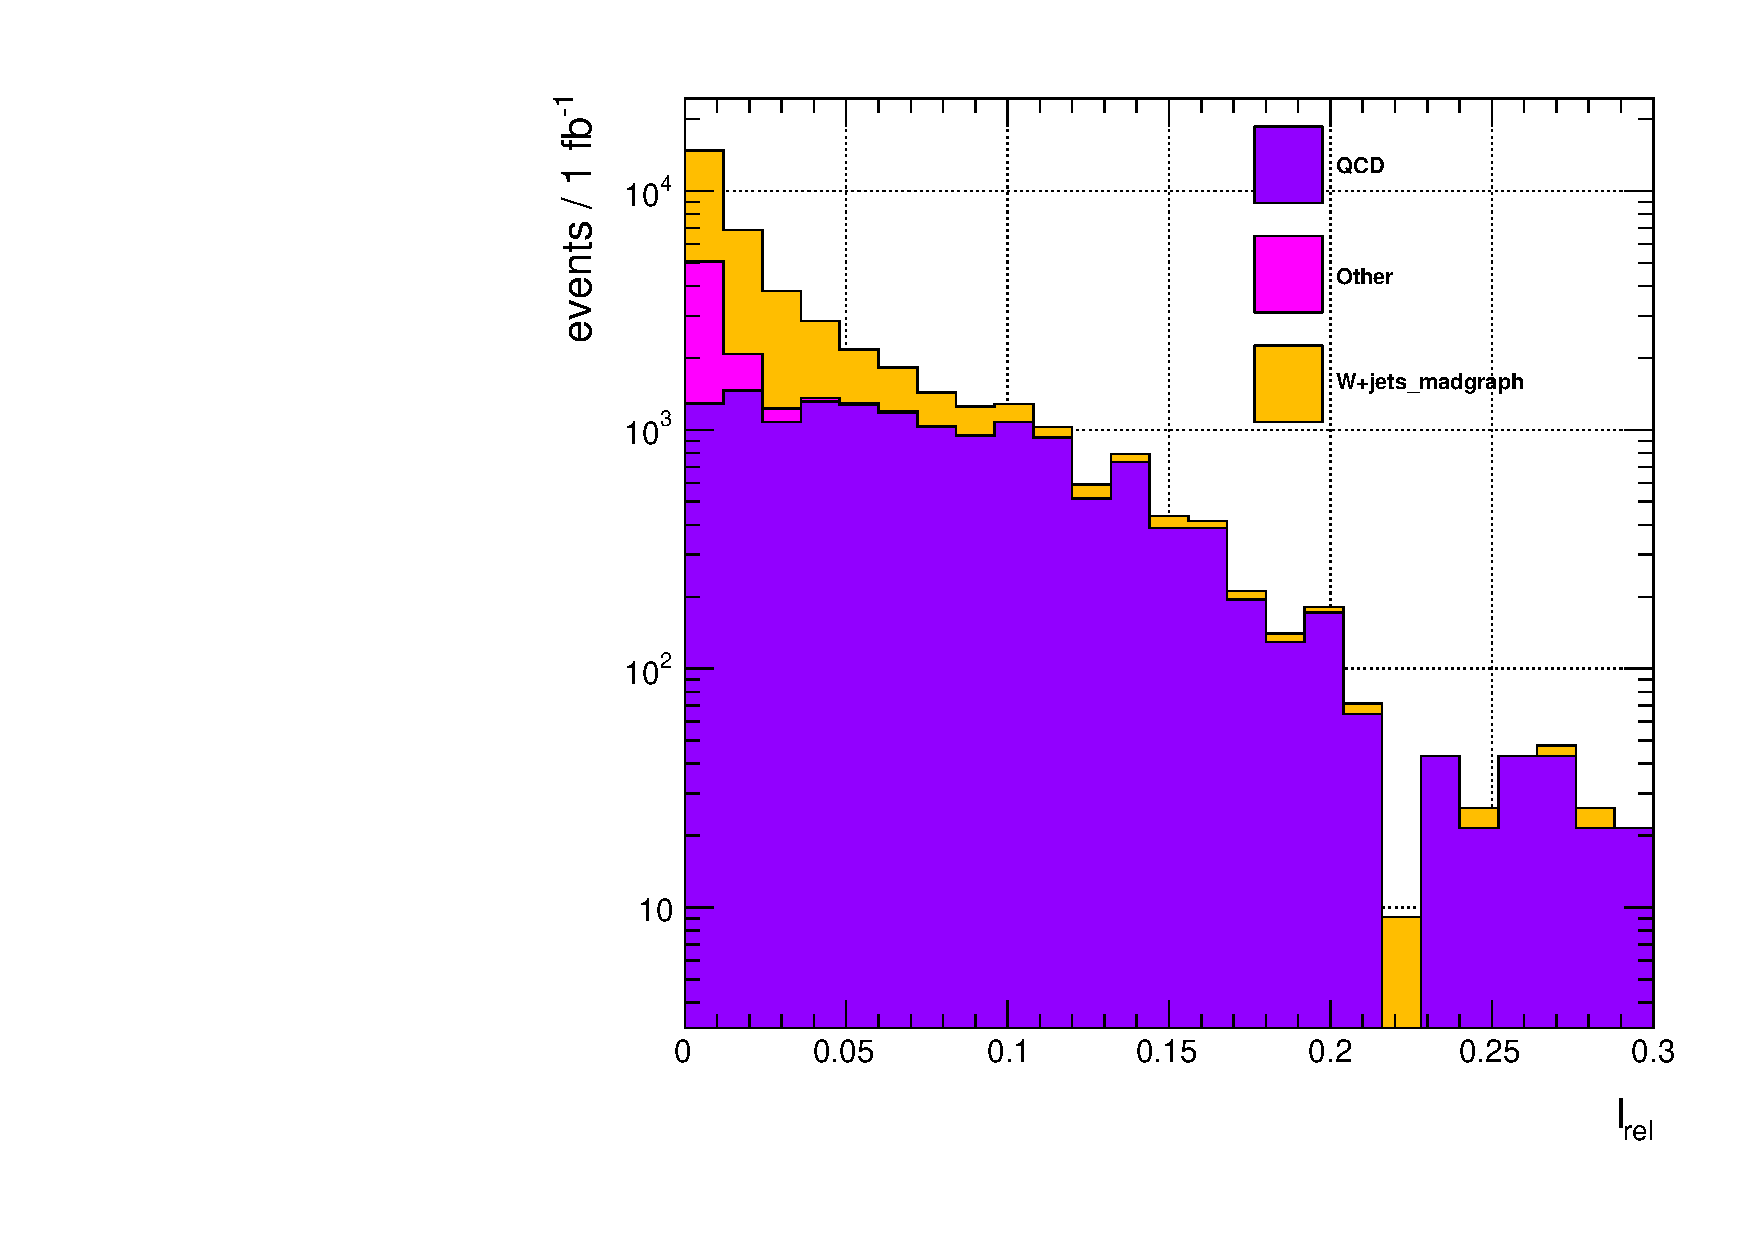
\includegraphics[width=0.45\textwidth]{plots/bkg_IsoStack.pdf}
    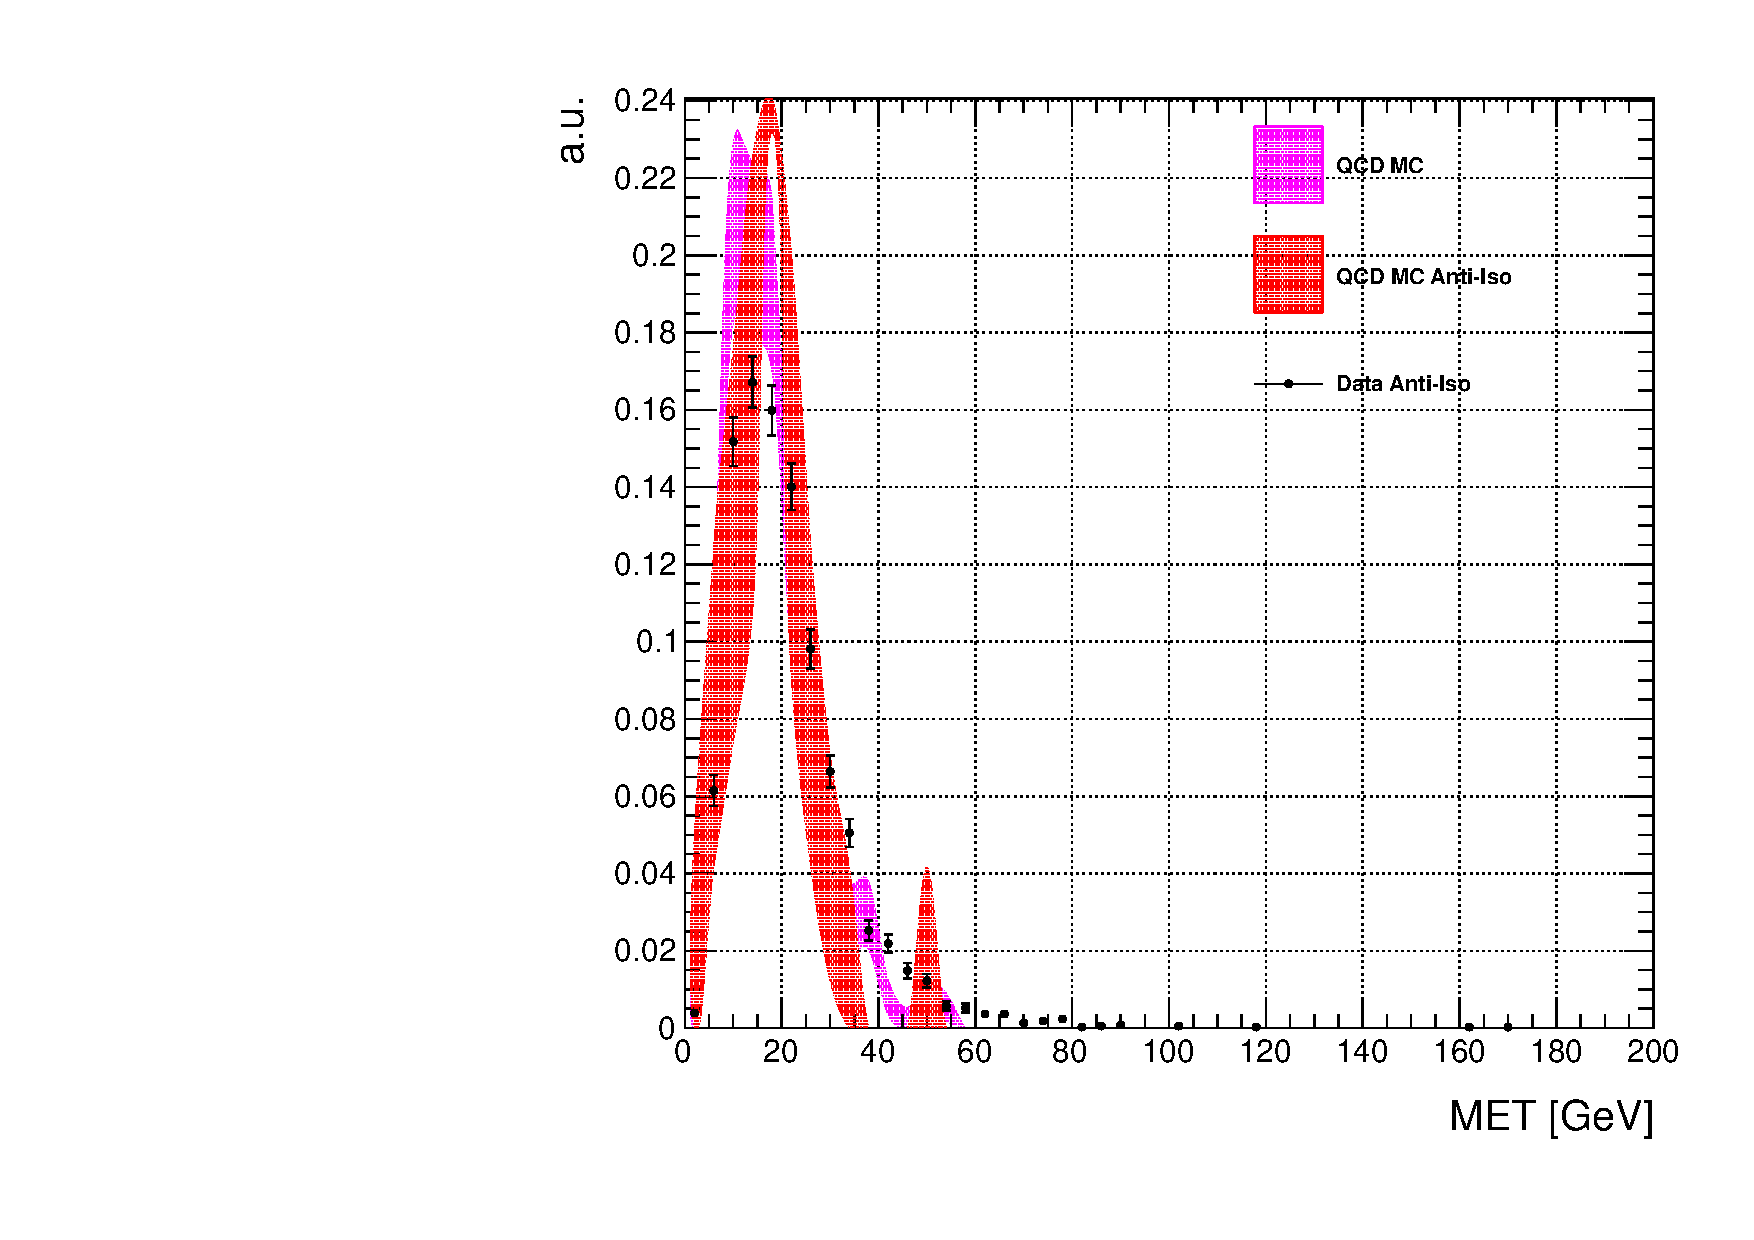
\includegraphics[width=0.45\textwidth]{plots/bkg_IsoShape.pdf}
    \caption{The $I_{rel}$ distribution (left) for the QCD, w+jets and other backgrounds from MC simulation. 
             Events are scaled to $1\ fb^{-1}$. \MET distributions (right) for the QCD in the Iso and Anti-Iso region 
             from MC simulations. Bands take into account statistical MC poissonian statistical fluctuation.
             Data in the control region for $950 pb^{-1}$ are superimposed.}
  \label{fig:bkg_QCD_IsoShape}
  \end{center}
\end{figure}

The fit of the \MET shape in the isolated region is shown in figure~\ref{fig:bkg_QCD_METStack}.
The fit is perfomed by maximizing a binned likelihood function, where all the PDFs are taken 
from MC, except the QCD that is obtained by inverting the isolation cut on the $950\ pb^{-1}$ 
sample of electron data. The free parameters of the fit are the QCD normalization and a global
normalization of the other backgrounds. The relative normalization of non-QCD events are taken
from MC.

To get the number of QCD events in the signal region, the fit distribution of the QCD events is integrated
in the $[30,\ +\infty)$ \MET range and the results are reported in table \ref{tab:bkg_QCD_DDYields}.

\begin{table}[htb]
  \begin{center}
  \begin{tabular}{c|c|c}
  \hline
         channel  & QCD MC expectation ($1\ fb^{-1}$) & QCD DD estimation ($1\ fb^{-1}$) \\
  \hline
  $e$    & \scriptsize{$(1.4\pm0.3)\cdot10^3$} & \scriptsize{$(3.3\pm0.1)\cdot10^3$}  \\
  \hline
  \end{tabular}
  \end{center}
  \caption{Expected number of QCD events for $1\ fb^{-1}$. The yields are shown for the pure
           MC expectation and the DD correction. Quoted errors take into account the MC statistics
           and the fit error respectively.}
  \label{tab:bkg_QCD_DDYields}
\end{table}
  
The error on the DD correction is taken from the likelihood function width. The method works with the first fraction of 
data sample since in that period the exploited triggers were not using any cut on the \MET; to get 
the contribution for the whole statistics we scale the results linearly with the luminosity.

To get the contribution of the QCD in the signal region defined in section \ref{sec:H0j_selections_intro} 
we scale the contribution evaluated with the presented method with the selection efficiency obtained
from the MC study.

\begin{figure}[h]
  \begin{center}
    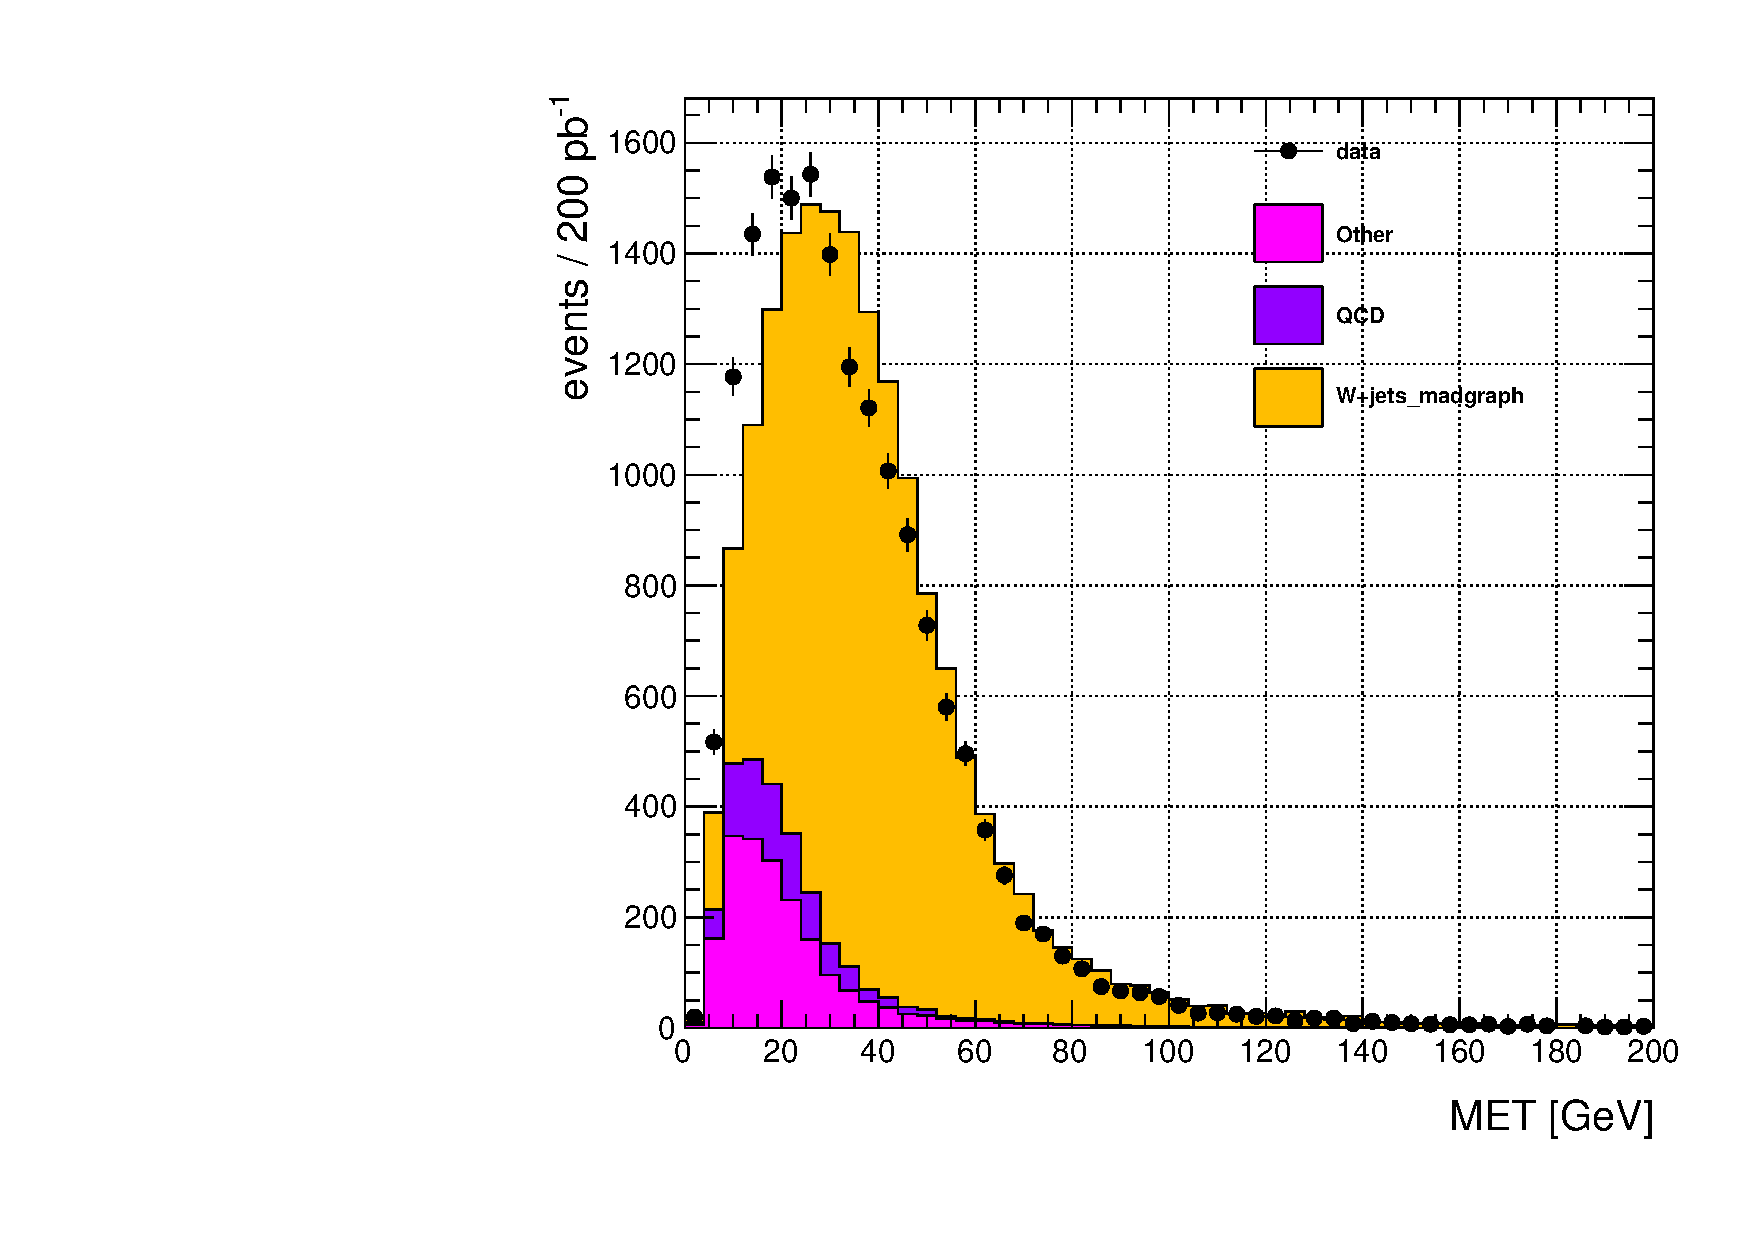
\includegraphics[width=0.45\textwidth]{plots/bkg_METStack_NoFit.pdf}
    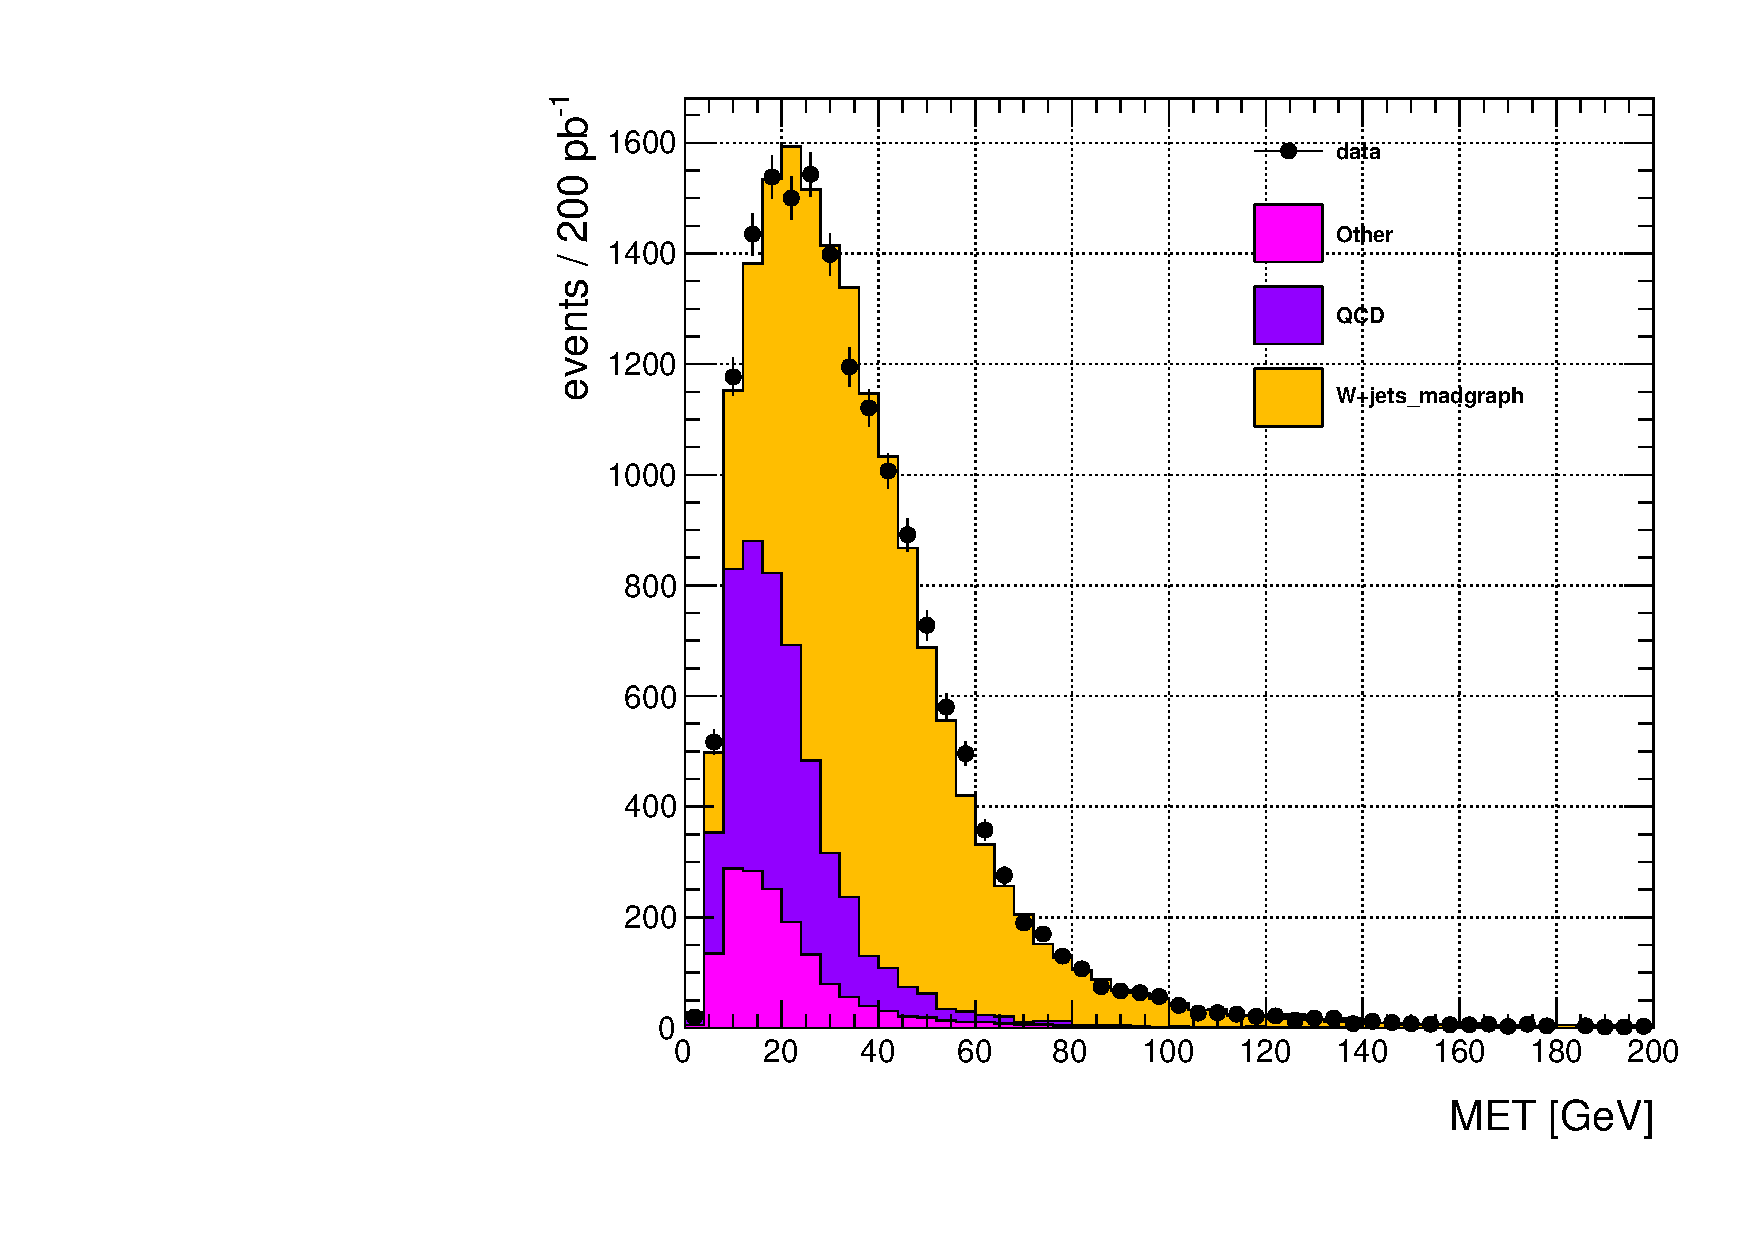
\includegraphics[width=0.45\textwidth]{plots/bkg_METStack.pdf}
    \caption{The DATA-MC comparison before (left) and after (right) the fit of 
             the \MET in the isolated region for the electrons. 
             The QCD shape is extracted from the non-isolated region.  
             while other processes shapes are taken from MC. MC is normalized to DATA.}
  \label{fig:bkg_QCD_METStack}
  \end{center}
\end{figure}

The contribution due to muon fakes is expected to be subleading with respect the electrons one, 
and considered negligible.
Figure \ref~{fig:blablabla} shows the distribution of events where leptons do not pass anti-isolation 
for muons (left) and electrons (right). \textbf{FIXME}

\subsection{ttbar}
% .... .... .... .... .... .... .... .... .... .... .... .... .... .... .... .... .... .... .... .... .... .... ....

The ttbar background contribution
is evaluated by using the Monte Carlo prediction of it.

\subsection{other backgrounds}
% .... .... .... .... .... .... .... .... .... .... .... .... .... .... .... .... .... .... .... .... .... .... ....


\section{Efficiencies and Systematic Uncertainties}
\label{sec:systematics}
\section{Other systematics sources}
\label{sec:systematics}
% ---- ---- ---- ---- ---- ---- ---- ---- ---- ---- ---- ---- ---- ---- ---- ---- ---- ---- ---- ---- ---- ---- ----


\subsection{Jet energy scale}
% .... .... .... .... .... .... .... .... .... .... .... .... .... .... .... .... .... .... .... .... .... .... ....


To evaluate the uncertainty due to jet energy scale in events with the
topology of this analysis, we reconstruct the hadronic W candidate
from an almost pure top data control sample.  A semileptonic top
sample is a good proxy for signal for the purposes of this study,
since the top quark pairs are produced by gluon fusion and decay to
two W bosons. These semileptonic top events are selected by requiring
exactly four jets in the event, out of which two are b-tagged and the
other two are anti-btagged. The hadronic W candidates are formed from
two anti-btagged jets.  The invariant mass of the hadronic W
candidates in the combined channels is shown in
Figure~\ref{fig:topw:muel}, for data and Monte Carlo, together with a
gaussian fit on the peak of each distribution.  The relative
difference between the gaussian means in data and Monte Carlo is used
as jet energy scale uncertainty, and propagated through the template
fits in the backgrounds, as well as to the signal shapes in the limit
setting. These results for 2012 are consistent with those found for
2011, when the typical effect was found to be of the order of less
than a percent.
%% as an example of signal shapes shown in Fig.~\ref{fig:sys:jesonsignal}.

\begin{figure}[htb] 
  {\centering
    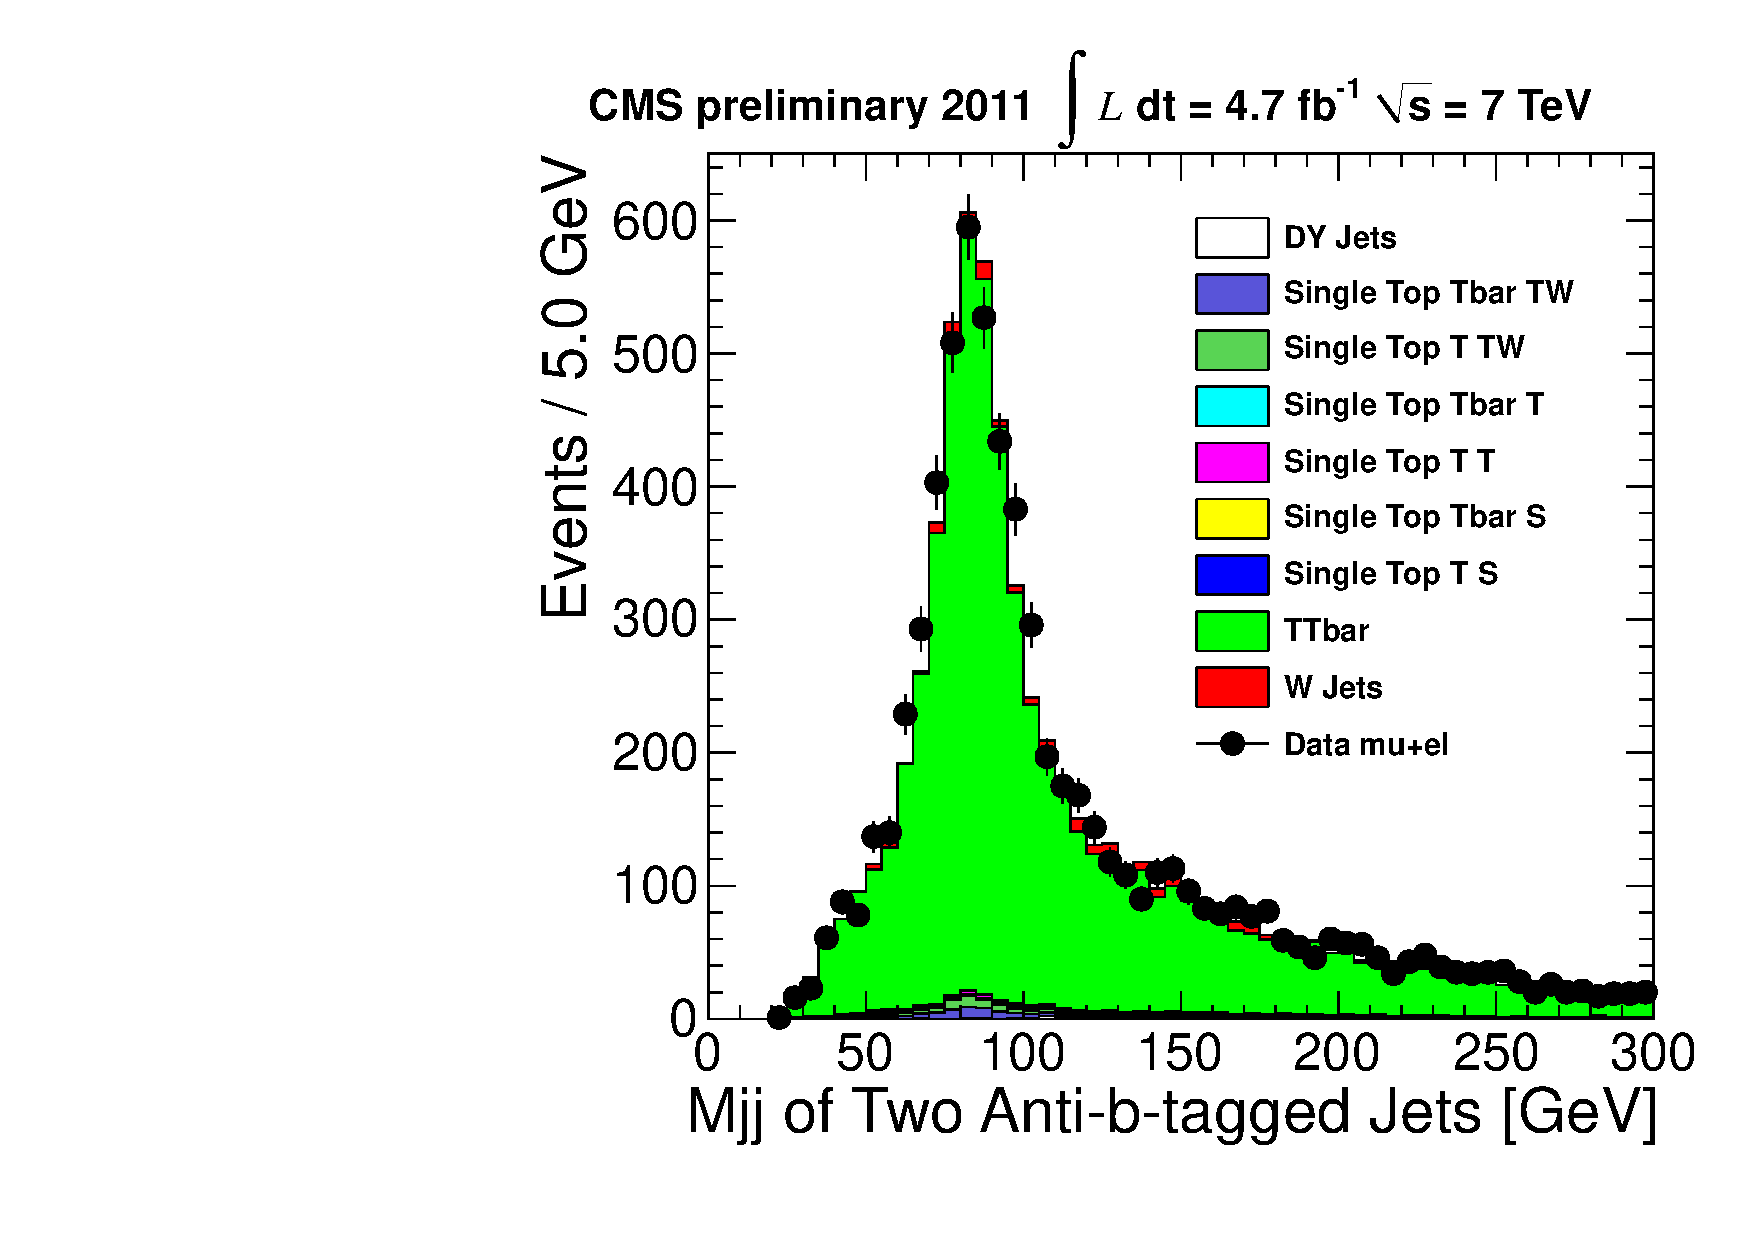
\includegraphics[width=0.325\textwidth]{plots/2012_JES/top_overlap_muel.pdf}
    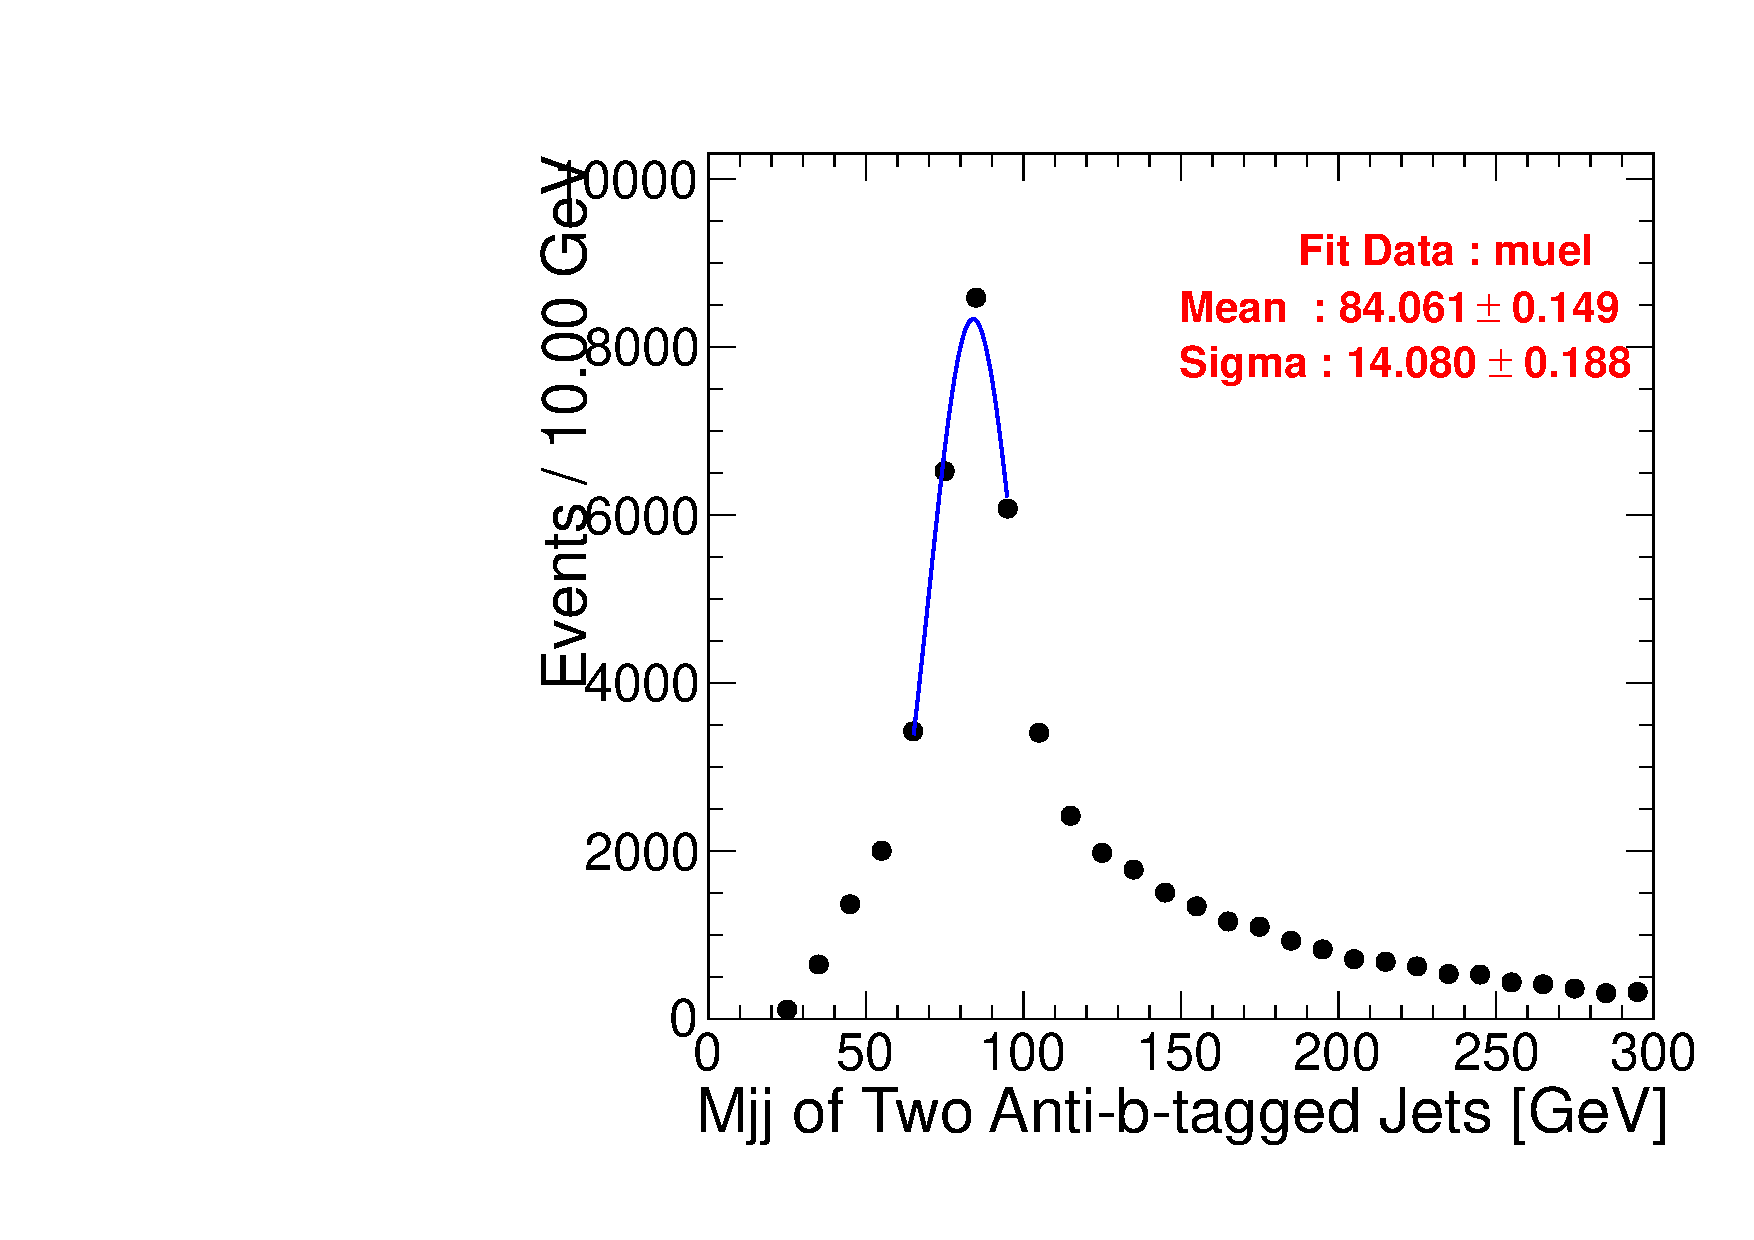
\includegraphics[width=0.325\textwidth]{plots/2012_JES/top_data_fit_muel.pdf}
    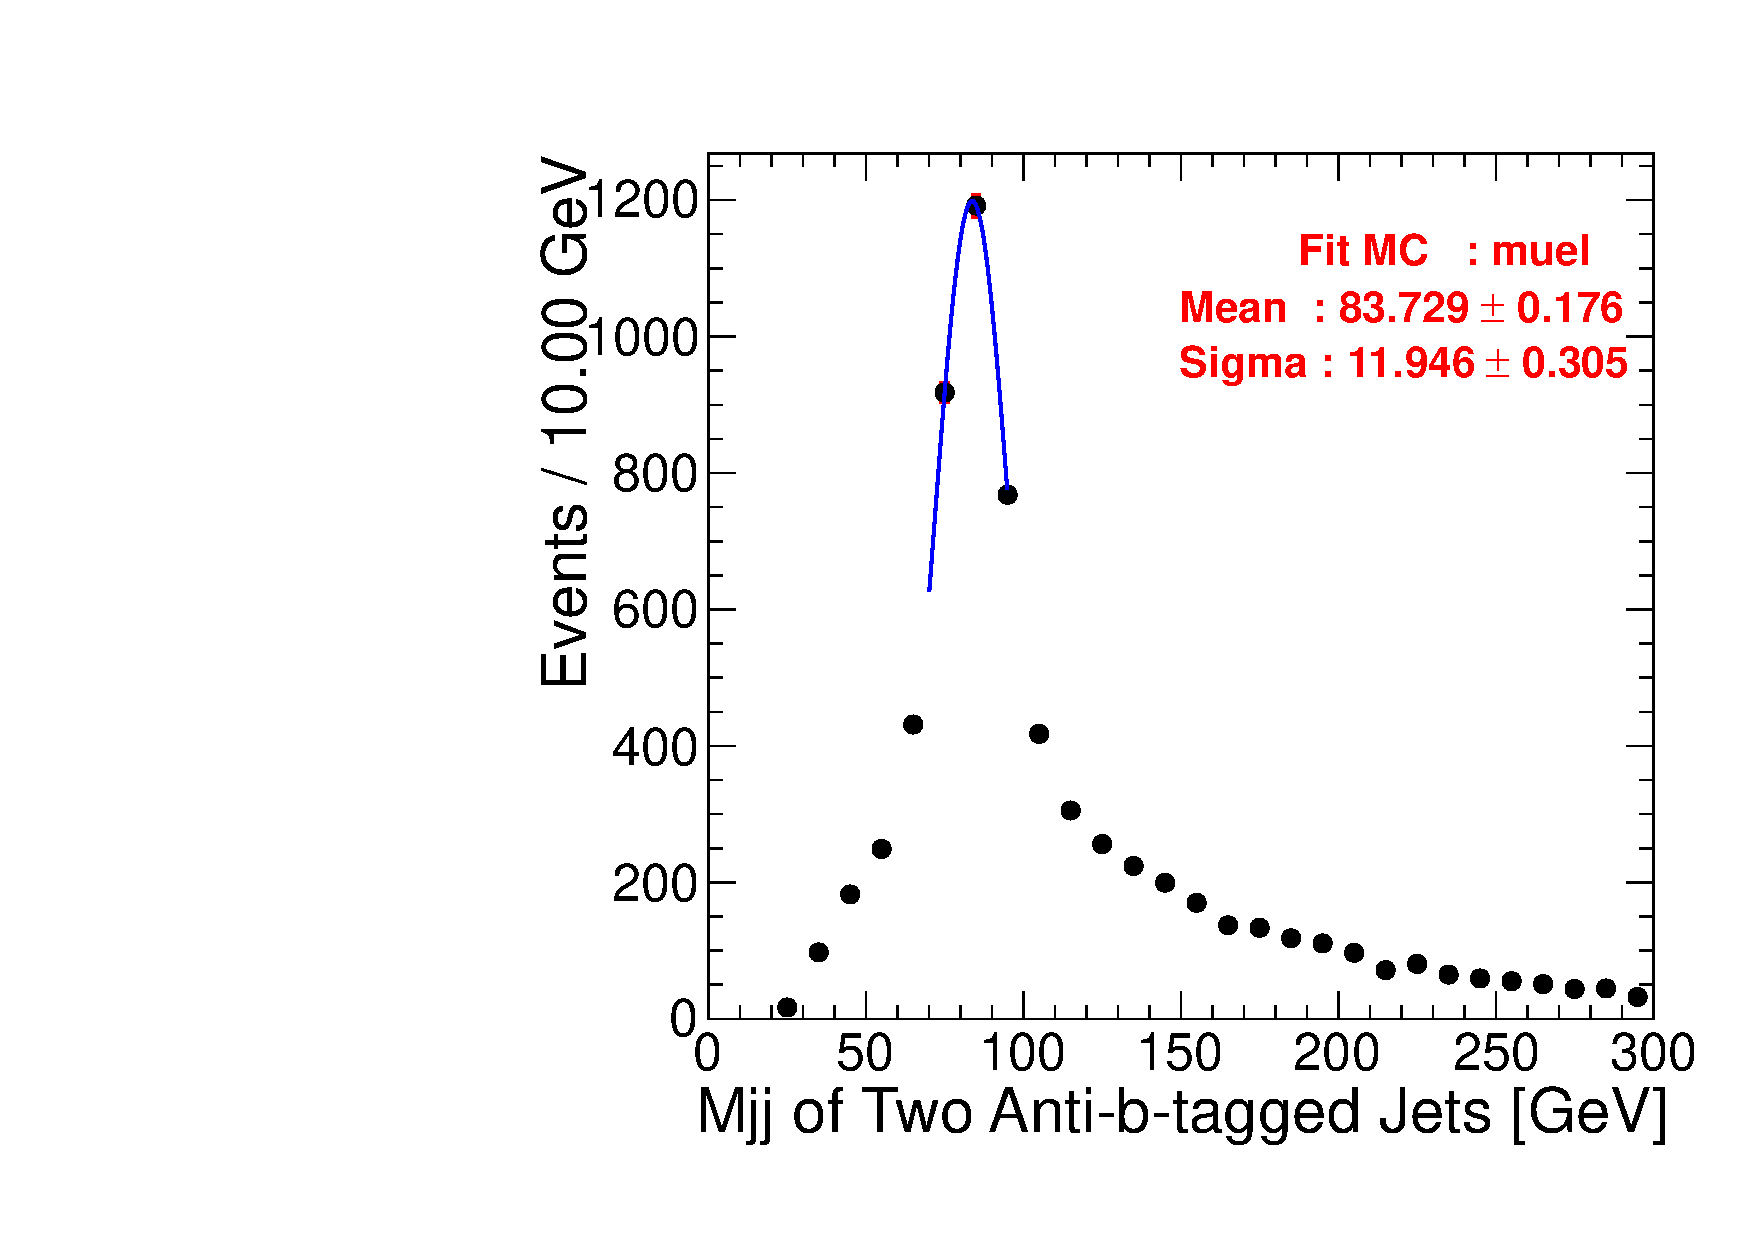
\includegraphics[width=0.325\textwidth]{plots/2012_JES/top_mc_fit_muel.pdf}
    \caption{The invariant mass distribution of the hadronic 
      W candidates in the semileptonic top sample (electron and 
      muon combined). 
      The left plot shows good agreement between the data and MC. 
      We fit the distribution with a Gaussian and extract the peak
      location for the data (middle) and MC (right).}
    \label{fig:topw:muel}}
\end{figure}

%% \begin{figure}[htb]
%%   \centering
%%   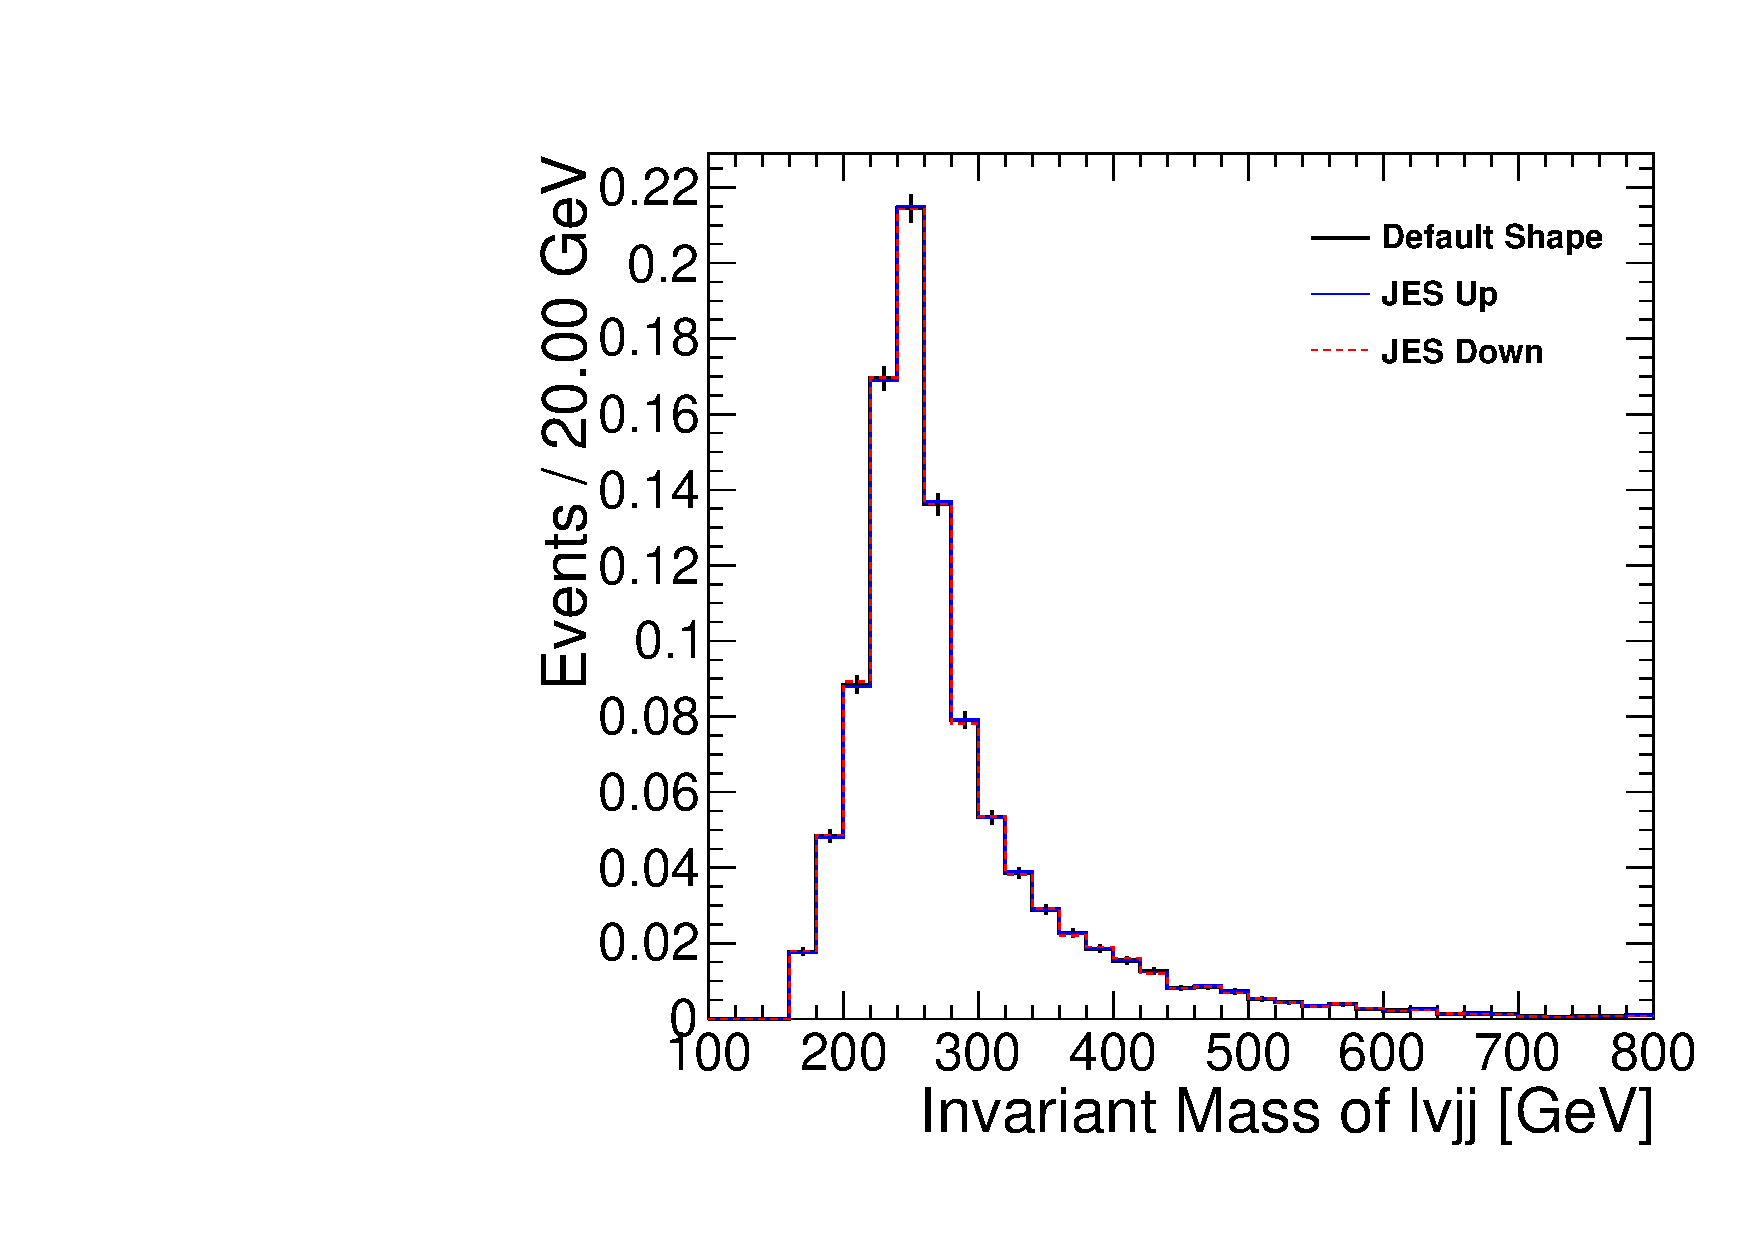
\includegraphics[width=0.49\textwidth]{plots/anaexample/sys-JES-mlvjj-mH250.pdf}
%%   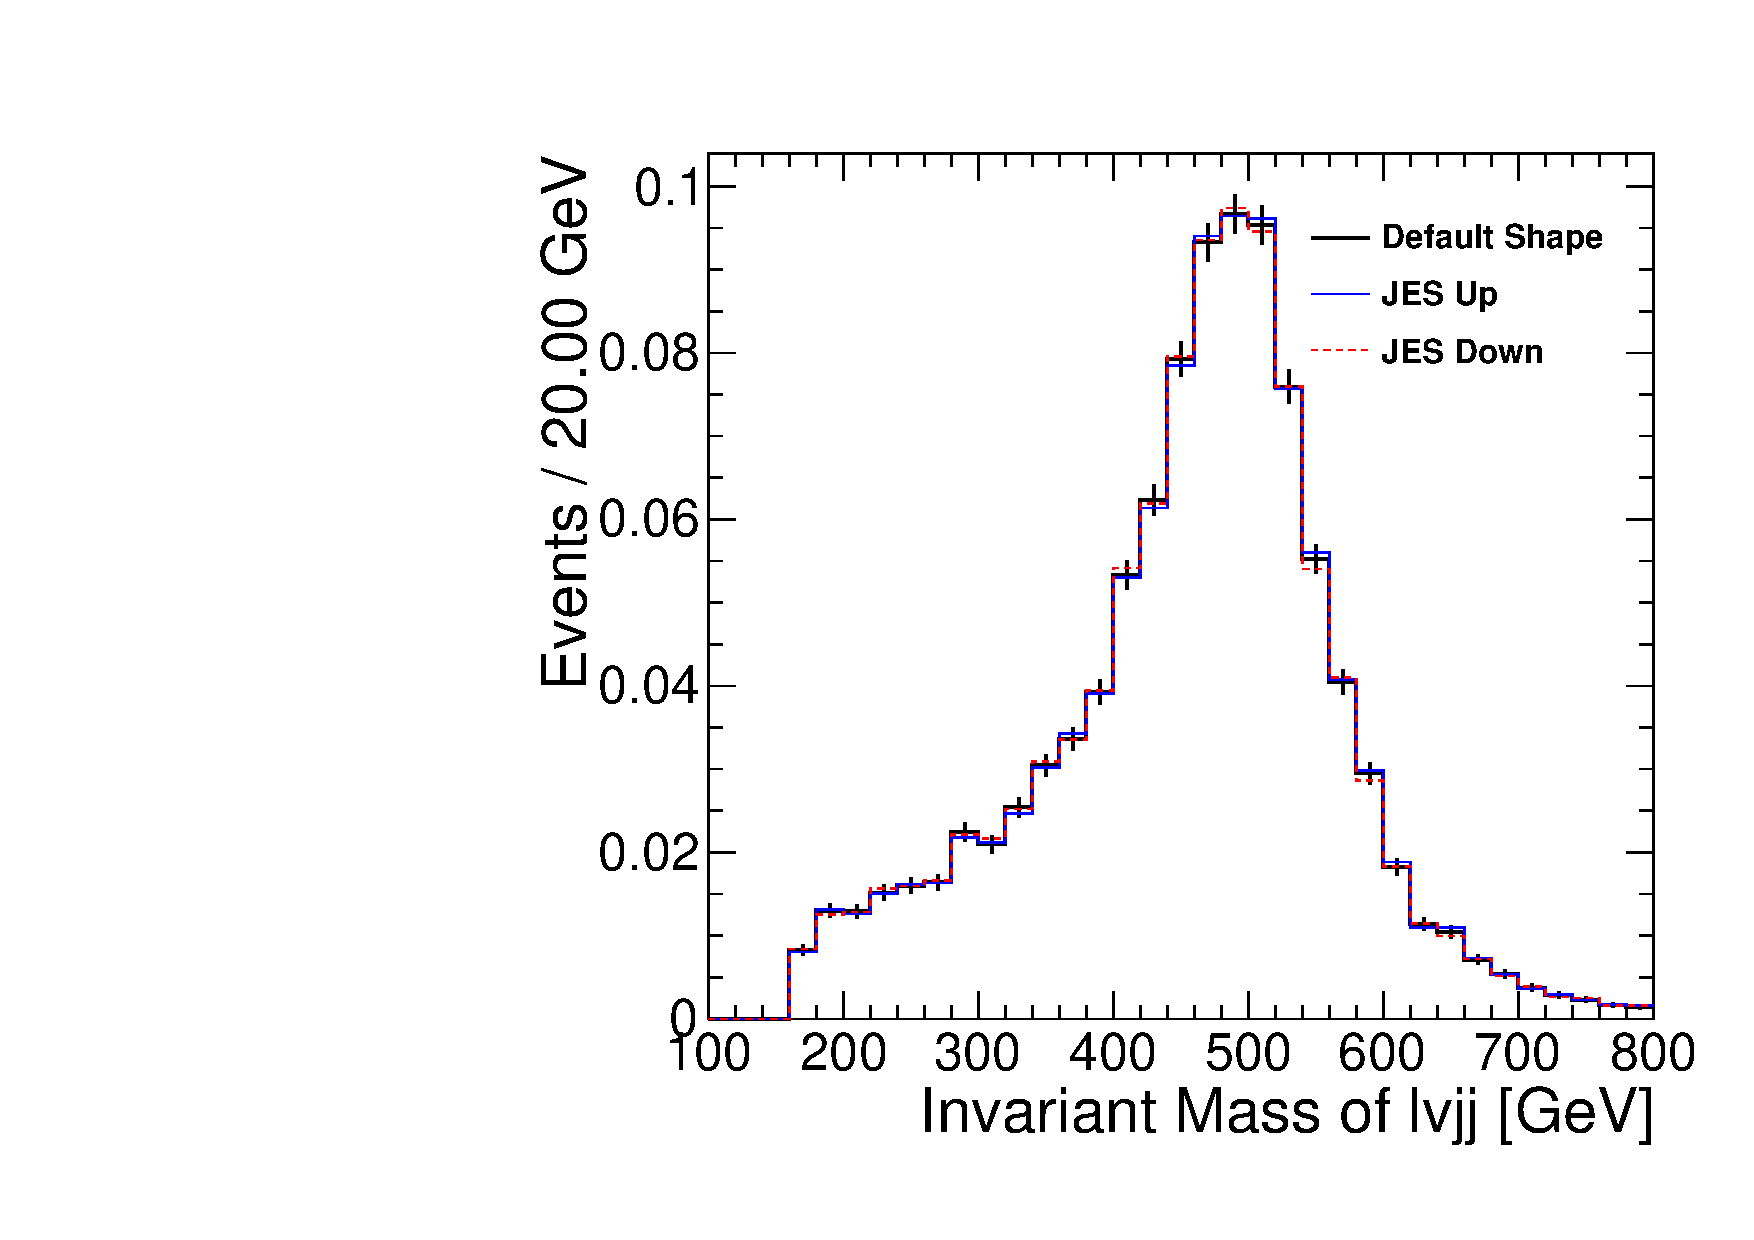
\includegraphics[width=0.49\textwidth]{plots/anaexample/sys-JES-mlvjj-mH500.pdf}
%%   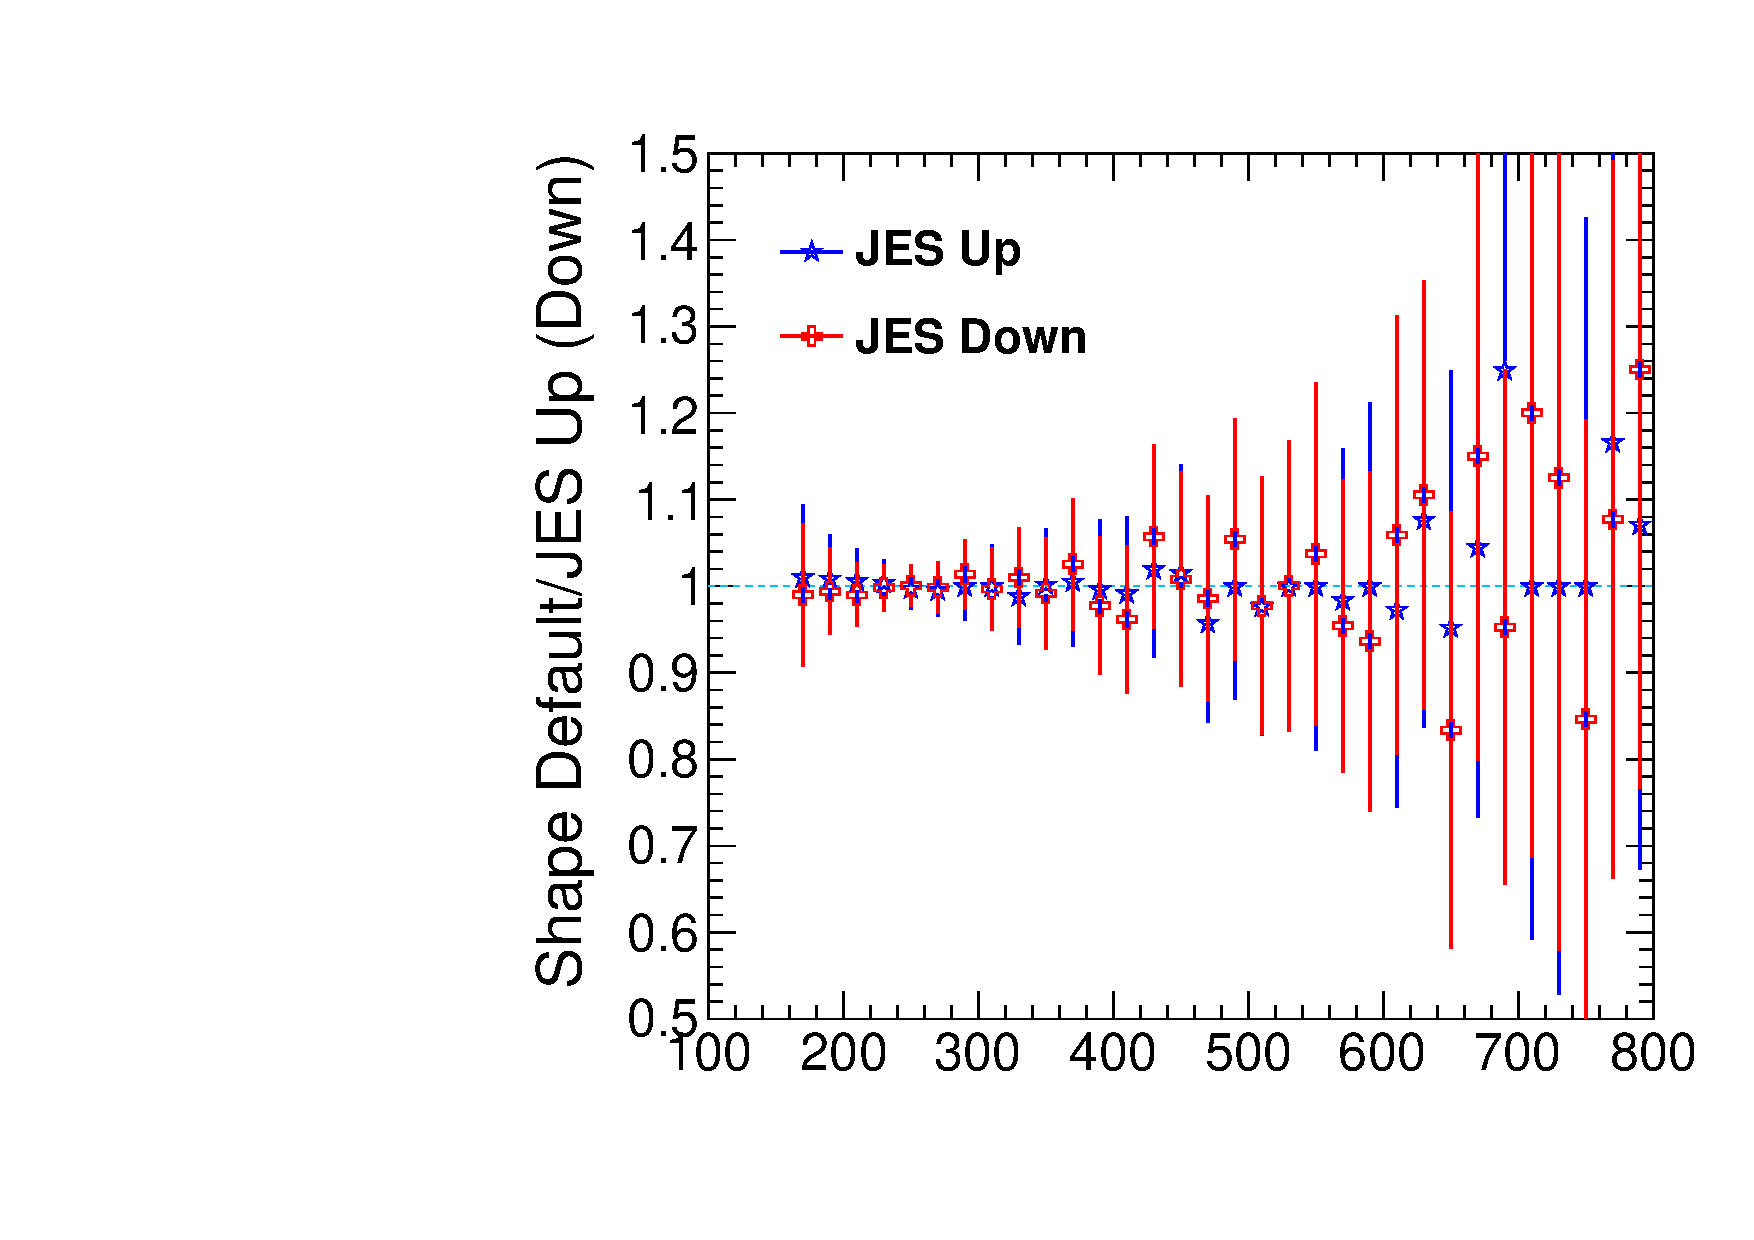
\includegraphics[width=0.49\textwidth]{plots/anaexample/sys-JES-ratio-mH250.pdf}
%%   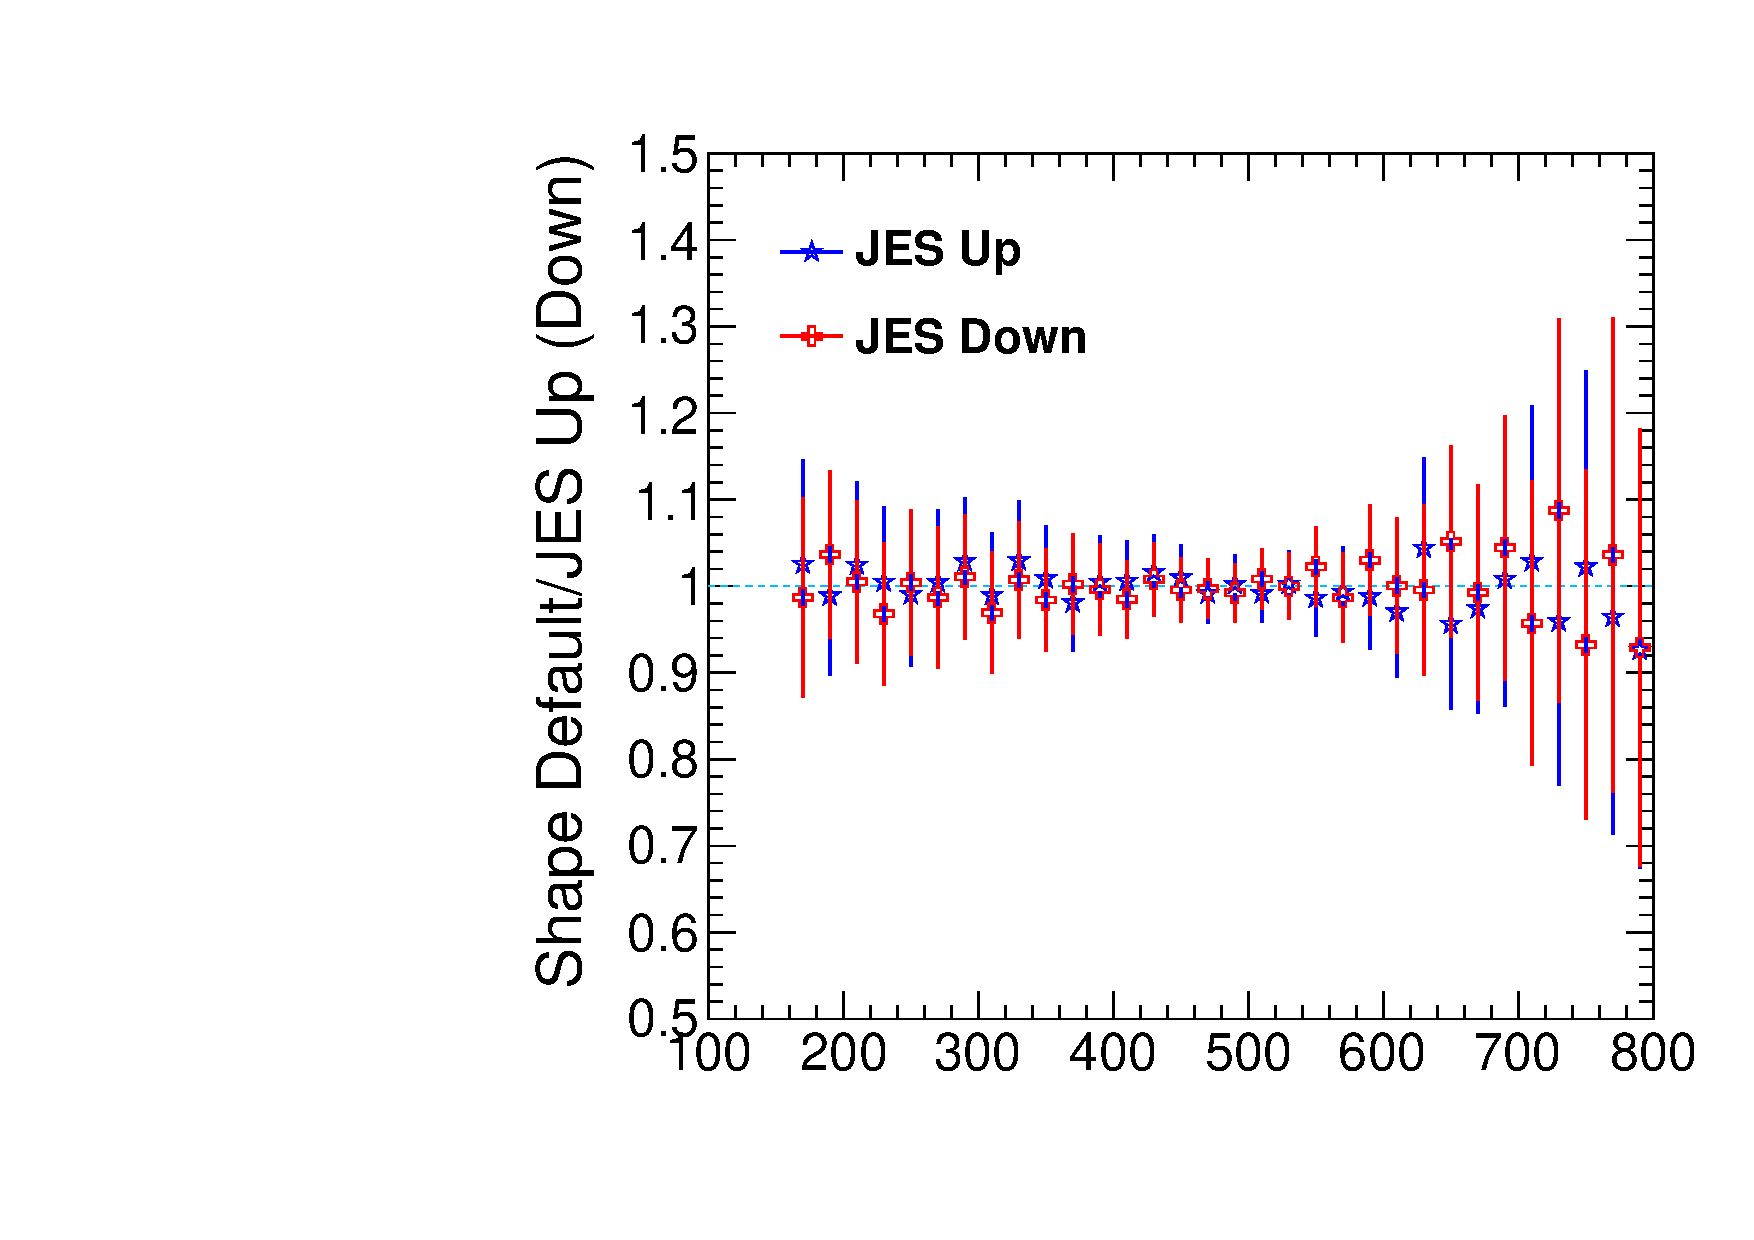
\includegraphics[width=0.49\textwidth]{plots/anaexample/sys-JES-ratio-mH500.pdf}
%%   \caption{\label{fig:sys:jesonsignal}The Higgs signal shape
%%     comparison between normal shape and the shape by shifting JES
%%     up/down by 0.5\%. The left plots are for Higgs mass 250~GeV and
%%     the right plots are for Higgs mass 500~GeV.}
%% \end{figure}

\subsection{Final selection efficiency on signal}

The systematic associated with the efficiency on the final selection
of the MVA output
%% and quark-gluon likelihood
is studied by using the same
top pair events as described above.  There is reasonable agreement
between the Monte Carlo and the data for the top sample. The
differences in selection efficiency are used to measure the potential
error in the signal efficiency for each mass point / channel
combination. The uncertainty is then taken as
\[
 100\% \times (1 - \frac{\epsilon_{data}}{\epsilon_{MC}}).
\]

The distribution of measured uncertainties per mass point/channel
combination is shown in Fig.~\ref{fig:sys:sigseleffuncdist}. The measured
efficiency uncertainties varied from less than 1\% to 10\%.
%% for masses where only the MVA output selection is in effect.
%% For those higher
%% masses for which the quark-gluon likelihood selection is also applied,
%% the largest variation was higher.
We therefore conservatively take 10\%
as the signal selection efficiency uncertainty for all channels and
mass points.
%% below the quark-gluon application cut-off, and 13\% as the
%% signal selection efficiency uncertainty for those channels and mass
%% points with quark-gluon likelihood selection applied.
We verified that
this conservative selection had no significant impact on the final
expected limit.

%% An alternative approach would be to reweight the signal Monte Carlo
%% samples according to the difference between data and Monte Carlo seen
%% in the MVA output distributions from the top samples, and then measure
%% the difference produced in the acceptance times efficiency.  This
%% cross check was performed for each channel/mass point combination, and
%% the distribution of changes are shown in
%% Fig.~\ref{fig:sys:sigseleffxcheck}. The spread of changes produced are
%% consistent with the systematics quoted above, which we retain as a
%% conservative estimate.

\begin{figure}[htb]
\center
%%\subfigure[
  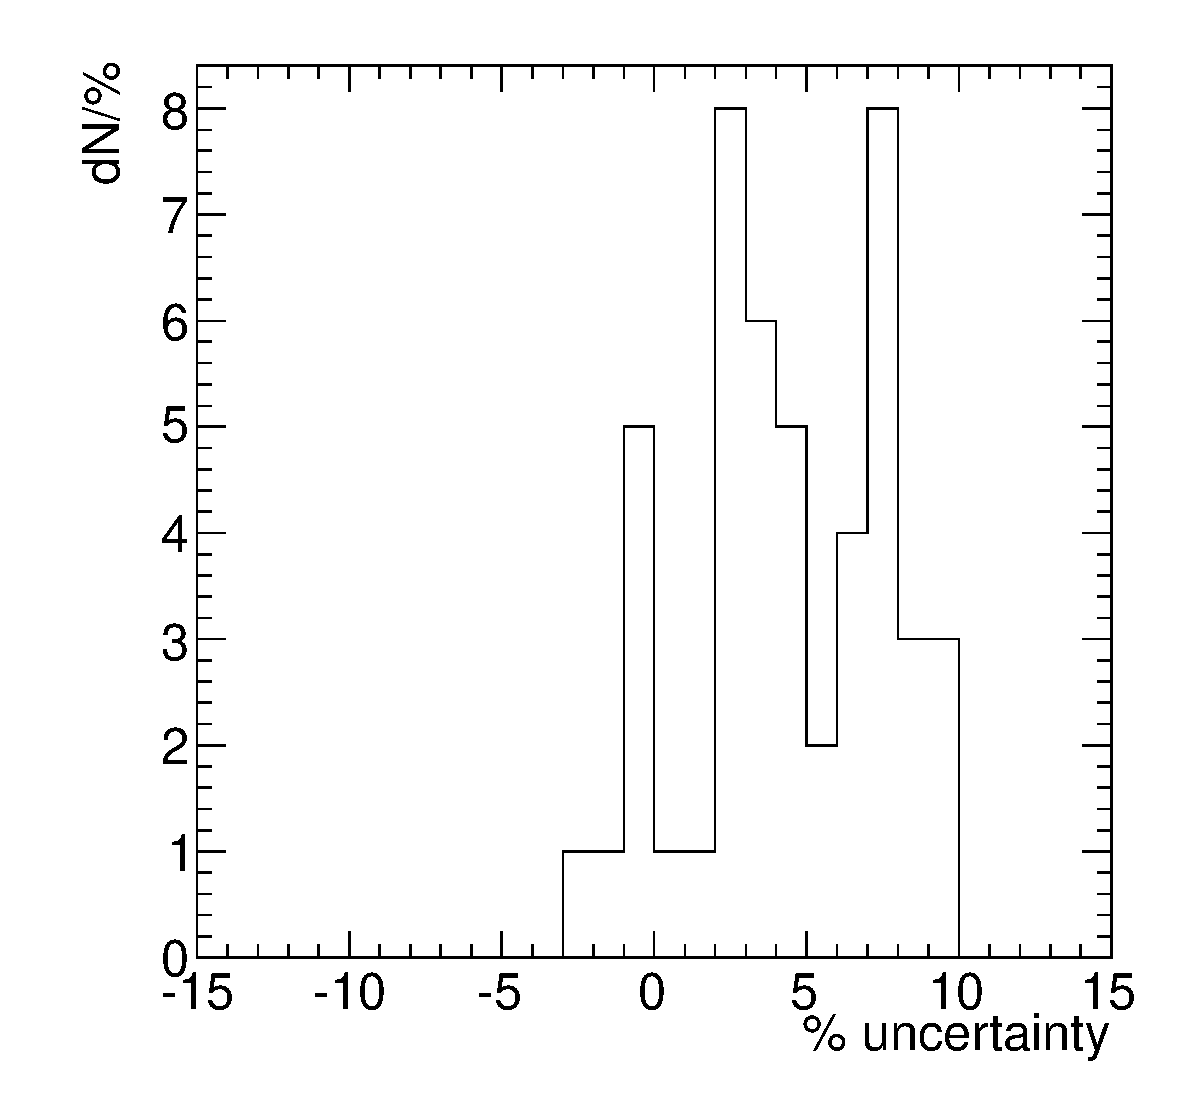
\includegraphics[width=0.49\textwidth]{plots/anaexample/sigseleffuncdist.pdf}
%% \subfigure[\label{fig:sys:sigseleffxcheck}] {
%%   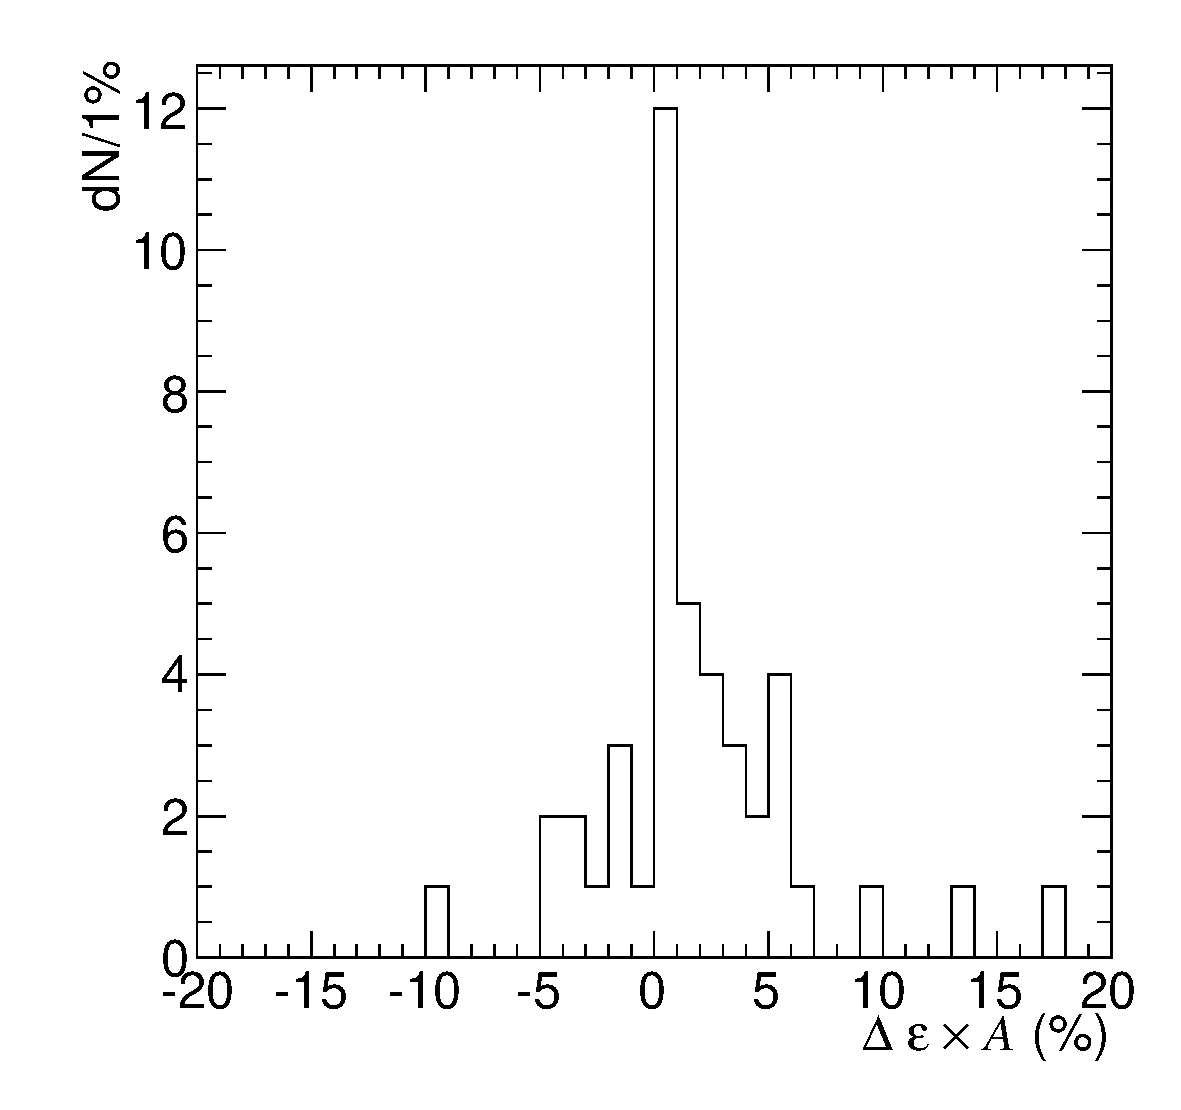
\includegraphics[width=0.49\textwidth]{plots/anaexample/sigseleffxcheckrewght.pdf}
%% }
  \caption{The distribution of measured uncertainties on signal
selection efficiency, one entry per channel/mass point
combination.
%% The uncertainties for high masses, for which the
%% quark-gluon likelihood discriminant is applied in addition to the MVA
%% discriminant, are shown in color.
%% b) The distribution, one entry per
%% channel/mass point, of the change in acceptance times efficiency
%% caused by reweighting the signal MC with the MVA output. The spread
%% is consistent with the quoted systematic.
}
\label{fig:sys:sigseleffuncdist}
\end{figure}

\subsection{Lepton selection and trigger efficiency}
%%.... .... .... .... .... .... .... .... .... .... .... .... .... .... .... .... .... .... .... .... .... .... ....
%%The lepton trigger and selection is common among several CMS analyses and 
%%we benefit from common studies based on tag-and-probe techniques. 
%%
Systematic uncertainties in the trigger efficiencies
are of the order of 1\%. Systematic uncertainties in the lepton reconstruction
and identification efficiency scale factors are of the order of 2\%. These uncertainties
are accounted for in the final systematics that are input to the limit setter.

\subsection{MET uncertainty}
% .... .... .... .... .... .... .... .... .... .... .... .... .... .... .... .... .... .... .... .... .... .... ....

MET directly affects our signal acceptance. 
The uncertainty prescription is discussed in Ref.~\cite{met}.
%https://twiki.cern.ch/twiki/bin/viewauth/CMS/MissingETUncertaintyPrescription
In addition, the MET distribution in the data is $\simeq$3\% wider 
than the MC, and placing a hard MET$>30.0$ cut creates an uncertainty. 
We estimate it by smearing the MET for each event by a Gaussian with 
a $\sigma =0.03*$MET and observing how many events pass the cut. 
Specifically, (Events Passing After Smearing)/(Events Passing Before Smearing) 
=0.998 for both muons and electrons.


\subsection{Pile-up model}
% .... .... .... .... .... .... .... .... .... .... .... .... .... .... .... .... .... .... .... .... .... .... ....


The average number of pile-up interaction in a given bunch crossing
BX$_{i}$ is given by the following formula:
\begin{equation}
N_{i} = \frac{\mathcal{L} \cdot \sigma_{\textnormal{min. bias}}}{\nu_{\textnormal{orbit}}},
\end{equation}
where $\mathcal{L}$ is the instantaneous luminosity,
$\sigma_{\textnormal{min. bias}}$ is the cross-section of minimum bias
interactions and $\nu_{\textnormal{orbit}}$ is the LHC orbit frequency
(11246~Hz).  Source of uncertainties in the estimation of the number
of pile-up interactions in data then come from the uncertainty on the
luminosity, currently $\textnormal{syst}_{\textnormal{lumi}}=5\%$ and
the uncertainty on the minimum-bias cross-section. We have adopted
$\sigma_{\textnormal{min. bias}}=69.3$~mb.

A total variation of 5\% in the number of interactions was propagated to the
re-weighting procedure for signal samples, and the obtained variation
in the signal yield is used as systematics on the signal. The typical
effect is less than a percent and therefore neglected.


\subsection{Cross-section prediction}
% .... .... .... .... .... .... .... .... .... .... .... .... .... .... .... .... .... .... .... .... .... .... ....


As of this writing, the inclusive cross-sections used for the Higgs
signal at 8~TeV center-of-mass energy have been calculated by the
Higgs Cross Section Working Group
\cite{LHCHiggsCrossSectionWorkingGroup:2011ti} for the
gluon-gluon fusion process, and have been used in the limits
extraction, together with their uncertainties, which are of the
order of 15-20\%. Equivalent cross-sections and uncertainties for the
vector boson fusion process have not yet been calculated, so the values
for 7~TeV center-of-mass energy scaled by a factor of 1.3 are used in
their place.

In addition, the acceptance effect due to the PDF choice has been
studyied by following the PDF4LHC recipe, that considers as
uncertainty the envelope of the error calculated for three sets of
PDFs \cite{Whalley:2005nh}, namely CT10, NNPDF and MSTW.
Table~\ref{tab:signalPDF} shows the values obtained.  For the purposes
of the limits calculation, these systematics are added in quadrature
to the inclusive cross-section uncertainties.
%
\begin{table}[h!t]
  \caption{Acceptance uncertainty related to the PDFs variation, 
           for the signal rate, as a function of the mass hypothesis.}
  \label{tab:signalPDF}
  \begin{center}
    \begin{tabular}{lc|lc}
      \hline
      \multicolumn{2}{c|}{ggF} & \multicolumn{2}{c}{VBF} \\
      \hline
      $m_{H}$ &  unc.   & $m_{H}$ &  unc.  \\
      \hline
%%       170  &  2.0\%  &  170  &  2.0\% \\ %FIXME conservative  
       180  &  2.0\%  &  180  &  2.0\% \\ %FIXME conservative  
%%       190  &  2.0\%  &  190  &  2.0\% \\ %FIXME conservative  
       200  &  2.0\%  &  200  &  2.0\% \\ %FIXME conservative  
%%       250  &  1.5\%  &  250  &  1.1\% \\  
       300  &  2.0\%  &  300  &  0.9\% \\  
%%       350  &  2.2\%  &  350  &  0.8\% \\  
       400  &  2.4\%  &  400  &  0.6\% \\  
       450  &  2.7\%  &  450  &  0.7\% \\  
       500  &  2.9\%  &  500  &  0.9\% \\  
       550  &  3.2\%  &  550  &  0.9\% \\  
       600  &  3.6\%  &  600  &  0.7\% \\  
      \hline
    \end{tabular}
  \end{center}
\end{table}

Eventually, an uncertainty is considered, in the case of gluon fusion
production, to account for the limitation of the narrow Higgs width
approximation in the Higgs simulation, and for the effect of
interference with Standard Model (SM) backgrounds.  The value used is
parametrized as a function of the Higgs mass as $150 \times m_H^3
[\%]$ where $m_H$ is expressed in TeV
\cite{Passarino:2010qk,Campbell:2011cu,Anastasiou:2011pi}.

Finally, there are uncertainties associated with the exclusive jet
binning used in this analysis. A detailed description of the source of
this uncertainty and how to calculate it is described in
\cite{cite:combine} Appendix C.  For this analysis we adopt the
numbers calculated by the $H\rightarrow WW\rightarrow 2\ell 2\nu$
group (\cite{cite:higgs2l2nu} Section~8.1).

\subsection{LHC luminosity}
% .... .... .... .... .... .... .... .... .... .... .... .... .... .... .... .... .... .... .... .... .... .... ....

The luminosity uncertainty has been considered 5\% \cite{lumiPAS}.

%%%%%%%%%%%%%%%%%%%%%%%%%%%%%%%%%%%%%%%%%%%%
\subsection{W+jets shape}
\label{sec:syst_mlvjj}
%%%%%%%%%%%%%%%%%%%%%%%%%%%%%%%%%%%%%%%%%%%%%
The $m_{\ell\nu jj}$ shape for W+jets events is taken from the data
sidebands. To get a smooth shape we parametrize this data-driven
shape using an exponential function. The decay parameter of this
parameterization has an associated error with it. We vary the
parameter up and down to get shape variations on the W+jets shape.
The shapes that are produced corresponding to the different systematic
variations on the parameters are propagated to the limit setting as a
systematic error.

The uncertainty on the $\alpha$ parameter used to combine the two
$m_{jj}$ sidebands would also constitute a variation in shape.  We
propagate the errors on alpha to the W+jets shape and combine its
effects on the shape with the uncertainty of the shape that arose
from the statistical power of the sideband data samples.

%%%%%%%%%%%%%%%%%%%%%%%%%%%%%%%%%%%%%%%%%%%%
\subsection{Background normalization}
\label{sec:syst_mjj}
%%%%%%%%%%%%%%%%%%%%%%%%%%%%%%%%%%%%%%%%%%%%%

The errors for the total background normalization are derived from the
unbinned maximum likelihood fit on the dijet invariant mass described
in Section~\ref{sec:mjjfitfornormal}. The non-Poisson fractional errors for
the 48 mass/lepton flavor/jet bin combinations are shown in
Table~\ref{tab:sys:normerrs}.  These are taken as a systematic
uncertainty on the background normalization in the signal region.

We compute these errors as
\[
\text{non-Poisson fractional error} \equiv \frac{\sqrt{\sigma_{N_\text{bkg}}^2-N_\text{bkg}}}{N_\text{bkg}}
\]
Poisson errors are included in the limit setting package.  We include
this additional systematic error which propagates additional
statistical errors derived in the dijet mass fit that are above and
beyond the Poisson errors alone.

\begin{table}[htb]
  \caption{Systematic uncertainties on the total background normalization.}
  \label{tab:sys:normerrs}
  \begin{center}
    \begin{tabular}{l|c|c|c|c} 
      \hline \hline
      $m_{\textnormal{H}}$  & electron 2-jet &electron 3-jet & muon 2-jet & muon 3-jet \\
      (\GeV)    & (\%)  &  (\%)  &  (\%)  &  (\%) \\\hline \hline
      180       &  0.6  &  0.5   &  0.4   &  0.4 \\
      200       &  0.7  &  0.9   &  0.4   &  0.5 \\
      300       &  0.6  &  0.9   &  1.0   &  0.9 \\
      400       &  0.9  &  2.1   &  0.7   &  1.8 \\
      450       &  1.1  &  2.2   &  1.4   &  3.1 \\
      500       &  1.1  &  0.0   &  1.4   &  0.0 \\
      550       &  1.0  &  3.1   &  1.5   &  0.0 \\
      600       &  1.2  &  4.0   &  1.3   &  0.0 \\
      \hline \hline
    \end{tabular}
  \end{center}
\end{table}

%  \subsection{Summary of systematic uncertainties}
%  % .... .... .... .... .... .... .... .... .... .... .... .... .... .... .... .... .... .... .... .... .... .... ....
%  
%  Table~\ref{tab:fitSystematics} summarizes all the sources of uncertainty considered.
%  %
%  \begin{table}[htb]
%    \begin{center}
%    \begin{tabular}{l|c|c}
%    \hline 
%    source                   &  impact on signal  &  impact on background \\
%    \hline
%    luminosity               &                    &            -          \\
%    cross-section            &                    &            -          \\
%    jet energy scale         &                    &                       \\
%    jet energy resolution    &                    &                       \\
%    unclustered met          &                    &                       \\
%    lepton energy scale      &                    &                       \\
%    trigger effiency         &                    &                       \\
%    lepton efficiency        &                    &                       \\
%    sideband fit             &         -          &                       \\
%    \hline
%    \end{tabular}
%    \end{center}
%    \caption{Sources of systematics considered in the fit analysis, with the corresponding value.}
%    \label{tab:fitSystematics}
%  \end{table}
%  %
%  
%  


\section{Results}
\label{sec:results}

Counting the number of events in the signal region,
the $\WW$ yield is calculated by subtracting the estimated contributions of the various 
SM background processes.  The signal efficiency times acceptance averaged over all 
lepton flavors including $\tau$s is found to be  $(3.22 \pm 0.22~\rm{(total)})\%$.

The total background yield is $275.2\pm 14.9~(\rm{stat.}) \pm 31.2~(\rm{syst.})$ 
events and the total number of
events observed is $1111$. Using the W $\to \ell \nu$ branching ratio of $(0.1080 \pm 0.0009)$ 
from Ref.~\cite{pdg}, the $\WW$ production cross section in pp collision data at 
$\sqrt{s} = 8~\TeV$, is calculated to be

\begin{displaymath}
\sigma_{\rm{WW}} = \measuredCrossSection.
\end{displaymath}

The statistical uncertainty is due to the total number of observed events.
The systematic uncertainty includes both the statistical and systematic 
uncertainties on the background prediction, as well as the uncertainty 
on the signal efficiency. This measurement is consistent with the 
SM expectation of~\nloCrossSection~\cite{MCFM}. The difference between the
measured and the theoretical value is $12.6 \pm 7.3$~pb, equivalent to
$(22 \pm 13)\%$ of the theoretical value. (Experimental and theoretical
uncertainties have been added in quadrature.)

%%% We have also measured the WW cross section in the di-lepton acceptance region,
%%% defined as follows: an event is accepted if the two leptons from the W bosons
%%% (be it electron, muon or tau) satisfy the $\pt > 20~\GeV$ and $|\eta| < 2.5$
%%% requirements. The acceptance defined this way has an efficiency of
%%% $\epsilon_{\rm{qq}} = 54.4$\% for the qq~$\to$~WW sample and
%%% $\epsilon_{\rm{gg}} = 61.8$\% for the gg~$\to$~WW sample. Using these values,
%%% together with $f_{\rm{gg}} = 0.03$, the WW fiducial cross section is
%%% %
%%% \begin{eqnarray}
%%%   \hat{\sigma}_{\rm{WW}} &=& \sigma_{\rm{WW}} \cdot {\rm{BR}}({\rm{WW}}\to\ell\nu\ell\nu) \cdot \left[f_{\rm{gg}}\cdot\epsilon_{\rm{gg}} + (1 - f_{\rm{gg}})\cdot\epsilon_{\rm{qq}}\right]\nonumber\\
%%%   ~\nonumber\\
%%%   ~ &=& 3.96 \pm 0.16~(\rm{stat.}) \pm 0.33~(\rm{syst.}) \pm 0.20~(\rm{lumi.})~\rm{pb.}\nonumber
%%% \end{eqnarray}

Finally, the measurement of the WW production cross section is interpreted in terms of the
ratio with the Z production cross section. The Z process is measured using events
passing the same lepton selection as the WW measurement, that fall within the Z
mass window in the ${\rm e}^+{\rm e}^-$ and $\mu^+\mu^-$ final states.
The theoretical expectation of the ratio $\sigma_{\rm{WW}}/\sigma_{\rm{Z}}$ at 8~TeV is
\mbox{$(1.72 \pm 0.08~(\rm{scale}) \pm 0.01~\rm({PDF}))\times 10^{-3}$}, where the
Z cross section at NNLO is calculated using \textsc{fewz}~\cite{FEWZ}. The efficiency
and the acceptance of the Z selection are obtained using the \textsc{madgraph} MC
sample, and the extrapolation factor to the $60~\GeV < m_{\ell\ell} < 120~\GeV$
mass range is obtained using \textsc{fewz}. The ratio of the $\WW$ 
efficiency times acceptance to the $\rm{Z}$ efficiency times acceptance is found 
to be $0.112 \pm 0.010~(\rm{syst.})$. The
systematic uncertainty on the efficiency ratio
takes into account the correlation between 
those uncertainties that are common to both terms.
By using the branching fraction for
${\rm{Z}}\to {\rm ee}/\mu\mu$ of $(6.73 \pm 0.008)\%$ from Ref.~\cite{pdg}, 
the WW to Z cross section ratio is found to be,

\begin{equation}
  \frac{\sigma(\rm{WW})}{\sigma(\rm{Z})} = (2.09 \pm 0.18~(\rm{syst.}) \pm 0.09~(\rm{stat.})) \times 10^{-3}.
\end{equation}

The systematic uncertainty includes the theoretical and experimental systematic uncertainties 
on the ratio of the efficiency times acceptance for the two processes, as well
as the total uncertainty due to the subtraction of background processes.
The statistical uncertainty is due to the total number of observed events.
The difference between the measured value of $\sigma_{\rm{WW}}/\sigma_{\rm{Z}}$
and the theoretical one is $(22\pm 13)\%$, neglecting correlations between 
theoretical uncertainties that contribute to both values.



\section{Conclusions}
\label{sec:conclusions}
This paper reports a measurement of the $\WW$ cross section in pp collisions at
$\sqrt{s} = 8~\TeV$. The measurement is performed in the $\WW\to\ell\nu\ell\nu$
decay channel, based on a total integrated luminosity of $\usedLumi$. The
measured cross section is \measuredCrossSection, to be compared with
the Standard Model NLO prediction of \nloCrossSection~\cite{MCFM}.


\section*{Acknowledgements}
We wish to congratulate our colleagues in the CERN accelerator departments for the excellent
performance of the LHC machine. We thank the technical and administrative staff at CERN and other CMS
institutes, and acknowledge support from: FMSR (Austria); FNRS and FWO (Belgium); CNPq, CAPES, FAPERJ,
and FAPESP (Brazil); MES (Bulgaria); CERN; CAS, MoST, and NSFC (China); COLCIENCIAS (Colombia); MSES
(Croatia); RPF (Cyprus); Academy of Sciences and NICPB (Estonia); Academy of Finland, MEC, and HIP
(Finland); CEA and CNRS/ IN2P3 (France); BMBF, DFG, and HGF (Germany); GSRT (Greece); OTKA and NKTH
(Hungary); DAE and DST (India); IPM (Iran); SFI (Ireland); INFN (Italy); NRF and WCU (Korea); LAS
(Lithuania); CINVESTAV, CONACYT, SEP, and UASLP-FAI (Mexico); MSI (New Zealand); PAEC (Pakistan);
MSHE and NSC (Poland); FCT (Portugal); JINR (Armenia, Belarus, Georgia, Ukraine, Uzbekistan); MON,
RosAtom, RAS and RFBR (Russia); MSTD (Serbia); MICINN and CPAN (Spain); Swiss Funding Agencies
(Switzerland); NSC (Taipei); TUBITAK and TAEK (Turkey); STFC (United Kingdom); DOE and NSF (USA).
Individuals have received support from the Marie-Curie programme and the European Research Council
(European Union); the Leventis Foundation; the A. P. Sloan Foundation; the Alexander von Humboldt
Foundation; the Belgian Federal Science Policy Office; the Fonds pour la Formation \`a la Recherche
dans l'\'industrie et dans l'\'Agriculture (FRIA-Belgium); the Agentschap voor Innovatie door Wetenschap
en Technologie (IWT-Belgium); the Council of Science and Industrial Research, India; and the HOMING
PLUS programme of Foundation for Polish Science, cofinanced from European Union, Regional Development
Fund.


%%% DO NOT ADD \end{document}!
%% **DO NOT REMOVE BIBLIOGRAPHY**
\bibliography{auto_generated}   % will be created by the tdr script.
